\documentclass[11pt,a4paper,reqno]{amsart}

\usepackage[utf8]{inputenc}
\usepackage[T1]{fontenc}
\usepackage{lmodern}
\usepackage{amsmath,amssymb,amsthm,mathtools}
\usepackage{booktabs}
\usepackage{array}
\usepackage{graphicx}
\usepackage{xcolor}
\definecolor{acadblue}{rgb}{0.0, 0.24, 0.52}
\usepackage[margin=2.45cm]{geometry}
\usepackage[colorlinks=true,linkcolor=acadblue,citecolor=acadblue,urlcolor=acadblue]{hyperref}

\newtheorem{theorem}{Theorem}[section]
\newtheorem{proposition}[theorem]{Proposition}
\newtheorem{lemma}[theorem]{Lemma}
\newtheorem{corollary}[theorem]{Corollary}
\theoremstyle{definition}
\newtheorem{definition}[theorem]{Definition}
\theoremstyle{remark}
\newtheorem{remark}[theorem]{Remark}

\numberwithin{equation}{section}
\allowdisplaybreaks
\emergencystretch=1.5em

\newcommand{\dd}{\mathrm{d}}
\newcommand{\ii}{\mathrm{i}}
\newcommand{\ee}{\mathrm{e}}
\newcommand{\Rea}{\operatorname{Re}}
\newcommand{\Ima}{\operatorname{Im}}
\newcommand{\Wig}{\mathcal{W}}
\newcommand{\Wtil}{\widetilde{W}}
\newcommand{\What}{\widehat{W}}
\newcommand{\sinch}{\operatorname{sinc}_{\mathrm{hyp}}}
\newcommand{\etah}{\eta_{\mathrm{hyp}}}
\newcommand{\fac}{\mathclose{\mathchar"0021}}

\title[Parity-Reduced Wronskians and Interval Enclosures for $\Xi$]{Parity-Reduced Transverse Wronskians, Jensen--Laguerre Moment Identities, and Division-Free Interval Enclosures for Riemann's $\Xi$-Function}

\author{Thijs Missiaen}
\address{Independent Researcher, Belgium (ORCID: 0009-0007-3678-0810)}
\email{thijs.missiaen@gmail.com}
\urladdr{https://orcid.org/0009-0007-3678-0810}

\subjclass[2020]{Primary 11M06, 65G30; Secondary 30D15, 26D15, 11Y35}
\keywords{Riemann Xi-function, parity-reduced transverse Wronskian, hyperbolic sinc kernel, Jensen--Laguerre invariants, Lehmer phenomenon, directed-rounding interval arithmetic, argument principle, catastrophic cancellation}

\date{October 2026}

\begin{document}

\begin{abstract}
Let $W(d,t) = \frac{1}{2}\partial_d|\Xi(t-\ii d)|^2$ be the transverse Wronskian of Riemann's completed function $\Xi(t-\ii d)$. Because $\Xi$ is real on $d = 0$, $W(-d,t) = -W(d,t)$ vanishes to odd order on the critical line, creating a $0/0$ degeneracy in interval enclosures touching $d = 0$. Factoring $d$ analytically via $\sinch(2dy) = \frac{\sinh(2dy)}{2dy}$ yields the canonical parity-reduced representation $\Wtil(d,t) = W(d,t)/d = 32\int_0^\infty y^2\sinch(2dy)I(y,t)\,\dd y$, whose Maclaurin coefficients $c_{2m-1}(t) = m\,L_m(\Xi;t)$ recover the classical differential invariants of Jensen (1913) and Csordas--Varga (1990), with $\Wtil(0,t) = L_1(\Xi;t) = (\Xi'(t))^2 - \Xi(t)\Xi''(t)$. Using positive-weight integral representations of $\sinch$ and $\etah$, we construct division-free Cauchy--Riemann gradients and non-harmonic-safe two-dimensional interval mean-value enclosures in \texttt{mpmath.iv}. As a methodological benchmark on $t \le 55$, we enclose $c_1, c_3, c_5 > 0$ at $\gamma_1, \dots, \gamma_{10}$, $80$ collar boxes around $\gamma_k$ and true $\Xi'$-extrema $\tau_k$, and five argument-principle rectangles, while demonstrating why IEEE-754 \texttt{float64} quadrature suffers $\ee^{+\pi t/4}$ roundoff amplification.
\end{abstract}

\maketitle

\section{Introduction}\label{sec:intro}

Let $\xi(s) = \frac{1}{2}s(s-1)\pi^{-s/2}\Gamma(s/2)\zeta(s)$ denote Riemann's completed zeta function, and write $s = \frac{1}{2} + d + \ii t$ with transverse offset $d = \sigma - \frac{1}{2} \in \mathbb{R}$ and spectral height $t \in \mathbb{R}$. Setting $z = -\ii(s - \frac{1}{2}) = t - \ii d$, Riemann's entire function $\Xi(z) := \xi(\frac{1}{2} + \ii z) = R(d,t) + \ii I_{\mathrm{im}}(d,t)$ admits the canonical Fourier--Laplace representation \cite{Riemann1859,Polya1926,Titchmarsh1986}
\begin{equation}\label{eq:Xi_integral}
\Xi(t - \ii d) = 8\int_0^\infty \Phi(u)\cosh(2d u)\cos(2t u)\,\dd u + \ii\,8\int_0^\infty \Phi(u)\sinh(2d u)\sin(2t u)\,\dd u,
\end{equation}
where the rapidly decaying Jacobi--Riemann kernel $\Phi(u)$ is given by
\begin{equation}\label{eq:Phi_def}
\Phi(u) := \sum_{n=1}^\infty \phi_n(u), \qquad \phi_n(u) := \left(2\pi^2 n^4 \ee^{9u} - 3\pi n^2 \ee^{5u}\right)\exp\!\left(-\pi n^2 \ee^{4u}\right).
\end{equation}
By the equivalence theorems of Hinkkanen \cite{Hinkkanen1997} and Lagarias \cite{Lagarias1999} (building on Speiser's geometric analysis of $\zeta'(s)$ \cite{Speiser1934}), the Riemann Hypothesis is equivalent to the positivity of $\Rea(\xi'(s)/\xi(s)) = W(d,t)/|\Xi(t-\ii d)|^2$ across the half-plane $d > 0$, where the \emph{transverse Wronskian} is given via the Cauchy--Riemann equations ($\partial_d R = \partial_t I_{\mathrm{im}}$, $\partial_d I_{\mathrm{im}} = -\partial_t R$) and the canonical Wigner correlation kernel $I(y,t) := \int_{-\infty}^\infty \Phi(\frac{x+y}{2})\Phi(\frac{x-y}{2})\cos(2t x)\,\dd x = 2\pi\,\Wig_\Phi(y/2, 2t)$ of Paper~I \cite{Missiaen2026Paper1} by
\begin{equation}\label{eq:W_def}
W(d,t) := \frac{1}{2}\frac{\partial}{\partial d}\big|\Xi(t-\ii d)\big|^2 = R\,\partial_t I_{\mathrm{im}} - I_{\mathrm{im}}\,\partial_t R = 16\int_0^\infty y\sinh(2d y)\,I(y,t)\,\dd y.
\end{equation}

When applying two-dimensional interval arithmetic near the critical line $d = 0$---an issue encountered in zero-free box computations for $\zeta'(s)$ and $\xi'(s)$ since Spira \cite{Spira1968,Spira1973}---one faces a kinematic \emph{boundary-layer degeneracy}: because $\Xi(t)$ is real-valued on $d = 0$, $I_{\mathrm{im}}(0,t) \equiv 0$ and $\partial_d R(0,t) \equiv 0$, forcing $W(0,t) \equiv 0$ identically for all $t \in \mathbb{R}$. Any naive interval box $\mathbf{B} = [0, \overline{d}] \times [\underline{t}, \overline{t}]$ touching $d = 0$ therefore contains zero in $W(\mathbf{B})$.

Analytically dividing $W(d,t)$ by $d$ leads directly to classical differential invariants. On the critical line $d = 0$, the limiting ratio $\lim_{d\to 0} W(d,t)/d = (\Xi'(t))^2 - \Xi(t)\Xi''(t)$ is the classical \emph{Laguerre expression} $L_1(\Xi;t)$, while the higher Maclaurin coefficients $c_{2m-1}(t) := \frac{1}{(2m-1)\fac}\partial_d^{2m-1}W(0,t)$ satisfy $c_{2m-1}(t) = m\,L_m(\Xi;t)$, where $L_m(f;t)$ are the higher Tur\'an--Jensen differential forms introduced by Jensen \cite{Jensen1913} in 1913 and proved by Csordas and Varga \cite{CsordasVarga1990} to satisfy $L_m(\Xi;t) > 0$ ($\forall\,m \ge 1$, $\forall\,t \in \mathbb{R}$) if and only if the Riemann Hypothesis holds (see also Griffin, Ono, Rolen, and Zagier \cite{Griffin2019} for asymptotic hyperbolicity of Jensen polynomials). Likewise, on the numerical side, the zeros of $\zeta(s)$ on $0 < t \le 55$ were already isolated over a century ago by Gram \cite{Gram1903} and extended by Titchmarsh and Comrie \cite{TitchmarshComrie1936}, Turing \cite{Turing1953}, and Platt and Trudgian \cite{PlattTrudgian2021} up to height $3 \cdot 10^{12}$.

The purpose of this note is accordingly twofold and strictly methodological: (i) to record the exact canonical Wigner-moment formulation of the parity-reduced Wronskian $\Wtil(d,t) := W(d,t)/d$, its Jensen--Laguerre Taylor coefficients, and division-free Cauchy--Riemann gradients with rigorous non-harmonic-safe Taylor bounds; and (ii) to benchmark directed-rounding interval enclosures (\texttt{mpmath.iv}) on $t \le 55$ while proving quantitatively via Higham's $|x|^\top|y|$ inner-product error bound why fixed-precision IEEE-754 \texttt{float64} quadrature breaks down exponentially at moderate heights.

\begin{theorem}[Canonical Parity-Reduced Wronskian, Jensen--Laguerre Moments, and Interval Enclosures]\label{thm:main}
Let $\Xi(t-\ii d) = R(d,t) + \ii I_{\mathrm{im}}(d,t)$ be defined by \eqref{eq:Xi_integral}, and let $I(y,t) = \int_{-\infty}^\infty \Phi(\frac{x+y}{2})\Phi(\frac{x-y}{2})\cos(2t x)\,\dd x$ be the canonical Wigner correlation kernel \cite{Missiaen2026Paper1}. Then:
\begin{enumerate}
\item[\textup{(i)}] \textbf{Odd parity reduction and canonical hyperbolic-sinc representation:} The transverse Wronskian satisfies $W(-d,t) = -W(d,t)$ with $\partial_d^{2k}W(0,t) \equiv 0$ for all $k \ge 0$. The parity-reduced Wronskian $\Wtil(d,t) := W(d,t)/d$ extends to an even real-analytic function on $\mathbb{R}^2$ given by
\begin{equation}\label{eq:W_tilde_thm}
\Wtil(d,t) = 32\int_0^\infty y^2\,\sinch(2d y)\,I(y,t)\,\dd y, \qquad \sinch(w) := \frac{\sinh w}{w} = \int_0^1 \cosh(s w)\,\dd s \ge 1,
\end{equation}
with flat Neumann tangent $\partial_d\Wtil(0,t) \equiv 0$ and boundary value equal to the classical Laguerre expression $\Wtil(0,t) = L_1(\Xi;t) := (\Xi'(t))^2 - \Xi(t)\Xi''(t)$.
\item[\textup{(ii)}] \textbf{Jensen--Csordas--Varga moment identity and local multiplicity jet:} The Maclaurin series $\Wtil(d,t) = \sum_{m=1}^\infty c_{2m-1}(t)\,d^{2m-2}$ has coefficients equal to $m$ times the Jensen--Laguerre invariant $L_m(\Xi;t)$ \cite{Jensen1913,CsordasVarga1990}:
\begin{equation}\label{eq:c_2m_thm}
c_{2m-1}(t) = \frac{2^{2m+3}}{(2m-1)\fac}\int_0^\infty y^{2m}I(y,t)\,\dd y = m\,L_m(\Xi;t) := m\sum_{j=0}^{2m}\frac{(-1)^{m+j}}{j\fac\,(2m-j)\fac}\,\Xi^{(j)}(t)\,\Xi^{(2m-j)}(t).
\end{equation}
At any $m$-fold real zero $t_0 \in \mathbb{R}$ ($\Xi(t_0) = \dots = \Xi^{(m-1)}(t_0) = 0$, $\Xi^{(m)}(t_0) \neq 0$), $c_1(t_0) = \dots = c_{2m-3}(t_0) = 0$ and $c_{2m-1}(t_0) = \frac{m}{(m\fac)^2}(\Xi^{(m)}(t_0))^2 > 0$. Across $\gamma_1, \dots, \gamma_{10}$, directed-rounding interval arithmetic (\texttt{mpmath.iv}) encloses $c_1(\boldsymbol{\gamma}_k), c_3(\boldsymbol{\gamma}_k), c_5(\boldsymbol{\gamma}_k) > 0$.
\item[\textup{(iii)}] \textbf{Non-harmonic-safe 2D Interval-MVT enclosures and \texttt{float64} cancellation obstruction:} Using the positive-weight integral representations of $\sinch(w)$ and $\etah(w) := \frac{w\cosh w - \sinh w}{w^3} = \int_0^1\int_0^1 s^2\cosh(s\tau w)\,\dd\tau\,\dd s$, all mixed $(d,t)$ partial derivatives of the non-harmonic auxiliary integrals in $\nabla\Wtil$ are bounded directly by holomorphic strip suprema of $\Xi^{(m)}$ without harmonicity assumptions. On the benchmark domain $t \in [0, 55]$, \texttt{mpmath.iv} (\texttt{iv.dps = 35}) encloses $\Wtil(\mathbf{B}_m).a > 0$ across $80$ collar boxes spanning $\gamma_1, \tau_1, \gamma_2, \tau_2, \gamma_3$ (with true $\Xi'$-roots $\tau_1 \approx 15.5857$, $\tau_2 \approx 22.0980$) and $N_{\mathrm{zeros}}(\Omega_k) = 0$ on five rectangles covering $[10^{-6}, 1.20] \times [0, 55]$. Conversely, IEEE-754 \texttt{float64} quadrature of $\What(d,t) = \ee^{\pi t/2}\Wtil(d,t)$ incurs roundoff error proportional to $u_{\mathrm{mach}}\ee^{+\pi t/4}$, reaching $4.51\%$ relative error at $t = 55$ and $1{,}375\%$ breakdown at $t = 60$.
\end{enumerate}
\end{theorem}

The principal benchmark constants verified in Sections~\ref{sec:dipole}--\ref{sec:numerics} are summarized below:
\begin{equation}\label{eq:canonical_constants}
\begin{aligned}
\Wtil(0,0) &= -\Xi(0)\Xi''(0) \approx 1.1420 \times 10^{-2}, \qquad
c_1(\gamma_1) = (\Xi'(\gamma_1))^2 \approx 1.9119 \times 10^{-6}, \\
c_3(\gamma_1) &= 2\,L_2(\Xi;\gamma_1) \approx 2.5881 \times 10^{-7}, \qquad
c_5(\gamma_1) = 3\,L_3(\Xi;\gamma_1) \approx 1.1553 \times 10^{-8}, \\
\tau_1 &= 15.58570859\dots, \quad \tau_2 = 22.09797728\dots \quad (\Xi'(\tau_k) = 0), \\
\min_{1\le m\le 80} \Wtil(\mathbf{B}_m).a &\approx +1.5592 \times 10^{-12} > 0, \qquad
\max_{1\le k\le 5} |N_{\mathrm{zeros}}(\Omega_k)| \le 2.62 \times 10^{-14} < \tfrac{1}{2}.
\end{aligned}
\end{equation}

Table~\ref{tab:literature} places these identities and interval benchmarks in the context of established prior work.

\begin{table}[htbp]
\centering
\caption{Relationship between classical prior art and the methodological contributions of this note.}\label{tab:literature}
\footnotesize
\begin{tabular}{p{0.27\textwidth} p{0.34\textwidth} p{0.32\textwidth}}
\toprule
\textbf{Prior Literature} & \textbf{Established Result} & \textbf{Contribution in This Note} \\
\midrule
Jensen (1913) \cite{Jensen1913}, P\'olya (1927) \cite{Polya1927}, Csordas--Varga (1990) \cite{CsordasVarga1990} & Differential invariants $L_m(f;t)$; equivalence $\mathrm{RH} \iff L_m(\Xi;t) > 0$ ($\forall\,m \ge 1$, $t \in \mathbb{R}$). & Identification $c_{2m-1}(t) = m\,L_m(\Xi;t) = \frac{2^{2m+3}}{(2m-1)\fac}\int_0^\infty y^{2m}I(y,t)\,\dd y$ and interval enclosures of $c_1, c_3, c_5 > 0$ at $\gamma_1, \dots, \gamma_{10}$. \\
\addlinespace[3pt]
Spira (1968--1973) \cite{Spira1968,Spira1973}, Hinkkanen (1997) \cite{Hinkkanen1997}, Lagarias (1999) \cite{Lagarias1999} & Positivity $\Rea(\xi'/\xi) > 0$ on $d > 0$; degeneracy $W(0,t) \equiv 0$ along $d = 0$. & Division-free gradient system $(\Wtil, \partial_t\Wtil, \partial_d\Wtil)$ via $\sinch$ and $\etah$ with non-harmonic-safe Taylor remainders on $[0, \overline{d}]$. \\
\addlinespace[3pt]
Gram (1903) \cite{Gram1903}, Titchmarsh--Comrie (1936) \cite{TitchmarshComrie1936}, Platt--Trudgian (2021) \cite{PlattTrudgian2021} & Verification of RH up to $T = 3 \cdot 10^{12}$ via Gram's law, Turing's method, and FFT interval arithmetic. & Methodological 2D collar + Cauchy winding benchmark on $t \le 55$ resolving true $\Xi'$-extrema $\tau_k$ vs.\ $Z'$-extrema. \\
\addlinespace[3pt]
Higham (2002) \cite{Higham2002}, Trefethen--Weideman (2014) \cite{TrefethenWeideman2014} & Inner-product error $|fl(x^\top y) - x^\top y| \le \gamma_N |x|^\top|y|$ and analytic strip trapezoidal convergence. & Quantitative proof that $\What_{\mathrm{float64}}$ suffers $\propto u_{\mathrm{mach}}\ee^{+\pi t/4}$ error amplification ($1{,}375\%$ error at $t = 60$). \\
\bottomrule
\end{tabular}
\end{table}

\subsection{Proof overview}\label{subsec:proof_overview}

The proof of Theorem~\ref{thm:main} proceeds in three steps:
\begin{enumerate}
\item \emph{Odd transverse parity and canonical hyperbolic-sinc kernel (Section~\ref{sec:parity}):} From Schwarz reflection $\Xi(t+\ii d) = \overline{\Xi(t-\ii d)}$, $|\Xi(t-\ii d)|^2$ is even in $d$ and $W(d,t)$ is odd in $d$. Dividing the canonical Wigner integral $W(d,t) = 16\int_0^\infty y\sinh(2dy)I(y,t)\,\dd y$ \cite{Missiaen2026Paper1} by $d$ and writing $\sinh(2dy)/d = 2y\sinch(2dy)$ yields \eqref{eq:W_tilde_thm} without $0/0$ division, valid identically for any real-entire Fourier transform.
\item \emph{Jensen--Laguerre Maclaurin hierarchy and division-free gradients (Section~\ref{sec:dipole}):} Expanding $\sinch(2dy)$ in powers of $(2dy)^2$ and matching with Leibniz differentiation of $\Xi(t-\ii d)\Xi(t+\ii d)$ recovers $c_{2m-1}(t) = m\,L_m(\Xi;t)$ \eqref{eq:c_2m_thm}. Differentiating $\sinch(w)$ via $\sinch'(w) = w\,\etah(w)$ yields division-free integral formulas for $\Wtil$, $\partial_t\Wtil$, and $\partial_d\Wtil$.
\item \emph{Non-harmonic-safe 2D Interval-MVT bounds and Higham cancellation audit (Sections~\ref{sec:interval}--\ref{sec:numerics}):} Because the division-free auxiliaries $\widetilde{I} = I_{\mathrm{im}}/d$ and $\widehat{I}_d$ do \emph{not} satisfy Laplace's equation $\partial_d^2 F = -\partial_t^2 F$, mixed $(d,t)$ Taylor remainders cannot be bounded by pure $t$-derivatives alone. Instead, expressing $\sinch(w) = \int_0^1 \cosh(sw)\,\dd s$ and $\etah(w) = \int_0^1\int_0^1 s^2\cosh(s\tau w)\,\dd\tau\,\dd s$ represents every partial derivative $\partial_d^p\partial_t^q F$ as a positive-weight average of the holomorphic derivatives $\Xi^{(m)}(t - \ii\delta)$ over $\delta \in [0, \overline{d}]$. We combine these enclosures with Cauchy's argument principle on $t \le 55$ and contrast them against the $\ee^{+\pi t/4}$ catastrophic cancellation of IEEE-754 \texttt{float64} quadrature.
\end{enumerate}

\subsection{Notation and conventions}\label{subsec:notation}

Throughout all papers in this series, we maintain a single canonical coordinate and normalization convention: $s = \sigma + \ii t = \frac{1}{2} + d + \ii t$ ($d = \sigma - \frac{1}{2} \in \mathbb{R}$, $t \in \mathbb{R}$), $z = -\ii(s-\frac{1}{2}) = t - \ii d$, and $\Xi(z) = \xi(\frac{1}{2}+\ii z)$ given by \eqref{eq:Xi_integral}--\eqref{eq:Phi_def}, so that $\Xi(t-\ii d) = 4\int_{-\infty}^\infty \Phi(u)\ee^{2(d+\ii t)u}\,\dd u$ and $\Xi(0) = \xi(\frac{1}{2}) \approx 0.4971207782$. The canonical mirror variables on $(u_1, u_2) \in \mathbb{R}^2$ are $x = u_1 + u_2$ and $y = u_1 - u_2$, with Wigner correlation kernel
\begin{equation}\label{eq:I_canonical_p2}
I(y,t) := \int_{-\infty}^\infty \Phi\!\left(\frac{x+y}{2}\right)\Phi\!\left(\frac{x-y}{2}\right)\cos(2t x)\,\dd x = 2\pi\,\Wig_\Phi\!\left(\frac{y}{2}, 2t\right),
\end{equation}
under which $|\Xi(t-\ii d)|^2 = 16\int_0^\infty \cosh(2dy)I(y,t)\,\dd y$, $W(d,t) = 16\int_0^\infty y\sinh(2dy)I(y,t)\,\dd y$, and $\Wtil(d,t) = 32\int_0^\infty y^2\sinch(2dy)I(y,t)\,\dd y$. (In terms of the rescaled coordinate $\tilde{y} = 2y$ and $\widetilde{\Phi}(w) = 2\Phi(w/2)$, the prefactor $32 y^2\,\dd y$ equals $\frac{1}{2}\tilde{y}^2\,\dd\tilde{y}$ with $\widetilde{I}(\tilde{y},t) = 8 I(\tilde{y}/2, t)$; we work exclusively with the canonical $(y, I(y,t))$ of \eqref{eq:I_canonical_p2} throughout.) We write $\What(d,t) := \ee^{\pi t/2}\Wtil(d,t)$ and $\widehat{c}_{2m-1}(t) := \ee^{\pi t/2}c_{2m-1}(t)$ for the Stirling-envelope-scaled fields. For a real interval $\mathbf{x} = [\underline{x}, \overline{x}]$, $\mathbf{x}.a := \underline{x}$, $\mathbf{x}.b := \overline{x}$, and $\operatorname{mid}(\mathbf{x}) := \frac{1}{2}(\underline{x}+\overline{x})$.

\section{Odd transverse parity and canonical hyperbolic-sinc representation}\label{sec:parity}

We first record the parity reduction of $W(d,t)$ in canonical Wigner coordinates, noting explicitly that this algebraic structure holds for any real-entire function $F(z)$ satisfying Schwarz reflection $F(\bar{z}) = \overline{F(z)}$ (whether or not $F$ satisfies the Riemann Hypothesis).

\begin{proposition}[Odd transverse parity and canonical Wigner--hyperbolic identity]\label{prop:parity_wigner}
For all $(d,t) \in \mathbb{R}^2$, the transverse Wronskian $W(d,t) = \frac{1}{2}\partial_d|\Xi(t-\ii d)|^2$ is an odd real-analytic function of $d$,
\begin{equation}\label{eq:odd_parity}
W(-d,t) = -W(d,t), \qquad \frac{\partial^{2k} W}{\partial d^{2k}}(0,t) \equiv 0 \quad (\forall\, k \ge 0).
\end{equation}
Consequently, the parity-reduced transverse Wronskian $\Wtil(d,t) := W(d,t)/d$ (with $\Wtil(0,t) := \partial_d W(0,t)$) is an even real-analytic function of $d$ satisfying the division-free phase-space identity
\begin{equation}\label{eq:boxed_wtilde}
\boxed{\Wtil(d,t) := \frac{W(d,t)}{d} = 32\int_0^\infty y^2\,\sinch(2d y)\,I(y,t)\,\dd y, \qquad \sinch(w) := \frac{\sinh w}{w} \ge 1.}
\end{equation}
In particular, $\partial_d\Wtil(0,t) \equiv 0$ for all $t \in \mathbb{R}$, and its critical-line value equals the classical Laguerre expression
\begin{equation}\label{eq:Wtil_d0}
\Wtil(0,t) = L_1(\Xi;t) := \big(\Xi'(t)\big)^2 - \Xi(t)\,\Xi''(t) = 32\int_0^\infty y^2\,I(y,t)\,\dd y.
\end{equation}
\end{proposition}

\begin{proof}
Since $\Phi(u)$ is real and even on $\mathbb{R}$, \eqref{eq:Xi_integral} implies $R(-d,t) = R(d,t)$ and $I_{\mathrm{im}}(-d,t) = -I_{\mathrm{im}}(d,t)$, i.e., $\Xi(t+\ii d) = \overline{\Xi(t-\ii d)}$. Hence $|\Xi(t-\ii d)|^2 = R(d,t)^2 + I_{\mathrm{im}}(d,t)^2$ is real-analytic and even in $d$, so $W(d,t) = \frac{1}{2}\partial_d|\Xi(t-\ii d)|^2$ is real-analytic and odd in $d$, yielding \eqref{eq:odd_parity}.

By \cite[Theorem~1.1(i)]{Missiaen2026Paper1}, changing variables $x = u_1 + u_2$, $y = u_1 - u_2$ (Jacobian $\frac{1}{2}$) in $|\Xi(t-\ii d)|^2 = 16\iint_{\mathbb{R}^2}\Phi(u_1)\Phi(u_2)\ee^{2d(u_1-u_2)}\cos(2t(u_1+u_2))\,\dd u_1\,\dd u_2$ gives
\begin{equation}\label{eq:Xi2_mirror_p2}
\big|\Xi(t-\ii d)\big|^2 = 16\int_0^\infty \cosh(2d y)\,I(y,t)\,\dd y.
\end{equation}
Because $|I(y,t)| \le I(y,0)$ decays super-exponentially ($\ll \ee^{8y}\exp(-2\pi\ee^{2y})$ as $y \to \infty$), $y^k\sinh(2D y)|I(y,t)| \in L^1([0,\infty))$ for every $D > 0$ and $k \ge 0$. Differentiating \eqref{eq:Xi2_mirror_p2} under the integral sign gives $W(d,t) = \frac{1}{2}\partial_d|\Xi(t-\ii d)|^2 = 16\int_0^\infty y\sinh(2d y)I(y,t)\,\dd y$. Dividing by $d \neq 0$ and inserting $\frac{\sinh(2d y)}{d} = 2y\sinch(2d y)$ yields \eqref{eq:boxed_wtilde}. Since $\sinch(w) = \sum_{m=0}^\infty \frac{w^{2m}}{(2m+1)\fac}$ is entire and even with $\sinch(0) = 1$, $\Wtil(d,t)$ is real-analytic and even in $d$ with $\partial_d\Wtil(0,t) = 0$. Finally, at $d = 0$, $I_{\mathrm{im}}(0,t) = 0$, $\partial_d R(0,t) = 0$, $\partial_d I_{\mathrm{im}}(0,t) = -\Xi'(t)$, and $\partial_d^2 R(0,t) = -\Xi''(t)$ by Cauchy--Riemann, so $\Wtil(0,t) = \partial_d(R R_d + I_{\mathrm{im}}I_{\mathrm{im},d})|_{d=0} = (\Xi'(t))^2 - \Xi(t)\Xi''(t)$, proving \eqref{eq:Wtil_d0}.
\end{proof}

\begin{remark}[Classical Laguerre inequality, Lehmer pairs, and off-line counterexamples]\label{rem:connections}
Identity \eqref{eq:Wtil_d0} clarifies both what parity reduction accomplishes and what it does \emph{not} prove unconditionally:
\begin{enumerate}
\item[\textup{(a)}] \emph{Laguerre's theorem vs.\ off-critical zeros:} For any real-entire function $F$ of genus $0$ or $1$ with \emph{only real zeros} (thus conditionally under RH for $\Xi$), Laguerre's classical theorem implies $L_1(F;t) = (F'(t))^2 - F(t)F''(t) \ge 0$ for all $t \in \mathbb{R}$, with strict inequality unless $t$ is a multiple zero \cite{Jensen1913,Polya1927,Csordas1986}. Conversely, if $F$ possesses a complex-conjugate pair of off-line zeros $t_* \pm \ii d_*$ ($d_* > 0$) near the real axis---as occurs unconditionally for the Davenport--Heilbronn function $\Xi_{\mathrm{DH}}(z)$ \cite{DavenportHeilbronn1936}---then $L_1(F; t_*)$ can become strictly negative (verified explicitly in Section~\ref{sec:scope}). Thus parity reduction removes the kinematic $0/0$ factor $d$, whereas global positivity $\Wtil(0,t) > 0$ remains a genuine spectral property.
\item[\textup{(b)}] \emph{Distinction between $\Xi'(t) = 0$ extrema, Hardy's $Z'(t) = 0$ extrema, and Gram points:} Writing $\Xi(t) = -\mathcal{A}(t) Z(t)$ with positive Archimedean envelope $\mathcal{A}(t) = \frac{1}{2}(\frac{1}{4}+t^2)\pi^{-1/4}|\Gamma(\frac{1}{4}+\frac{\ii t}{2})| \asymp \frac{t^2}{\sqrt{2}}(\frac{2\pi}{t})^{1/4}\ee^{-\pi t/4}$, differentiation gives $\Xi'(t) = -[\mathcal{A}'(t)Z(t) + \mathcal{A}(t)Z'(t)]$. Because $\mathcal{A}'(t)/\mathcal{A}(t) \approx -\frac{\pi}{4} + \frac{7}{4t} < 0$ for $t \ge 3$, the critical-line extrema $\tau_k$ solving $\Xi'(\tau_k) = 0$ are shifted substantially leftward relative to both the extrema of $Z(t)$ ($t_{Z',1} = 17.88258208\dots$, $t_{Z',2} = 23.10465065\dots$) and the Gram points ($g_0 = 17.84559954\dots$, $g_1 = 23.17028270\dots$): the first two positive roots of $\Xi'(\tau_k) = 0$ lie at $\tau_1 = 15.58570859\dots$ and $\tau_2 = 22.09797728\dots$. At $\tau_k$, $(\Xi'(\tau_k))^2 = 0$ and $\Wtil(0,\tau_k) = -\Xi(\tau_k)\Xi''(\tau_k)$ isolates the local concavity barrier studied by Lehmer \cite{Lehmer1956}.
\end{enumerate}
\end{remark}

\section{Jensen--Laguerre moment hierarchy and division-free Cauchy--Riemann gradients}\label{sec:dipole}

Expanding $\sinch(2dy)$ around $d = 0$ identifies the transverse Taylor coefficients of $\Wtil(d,t)$ with the higher differential invariants of Jensen \cite{Jensen1913} and Csordas--Varga \cite{CsordasVarga1990}.

\begin{theorem}[Jensen--Csordas--Varga moment hierarchy and local multiplicity jet]\label{thm:dipole_hierarchy}
For every $t \in \mathbb{R}$, the parity-reduced Wronskian $\Wtil(d,t)$ expands as the convergent Maclaurin series in $d^2$,
\begin{equation}\label{eq:Wtil_taylor}
\Wtil(d,t) = \sum_{m=1}^\infty c_{2m-1}(t)\,d^{2m-2} = c_1(t) + c_3(t)\,d^2 + c_5(t)\,d^4 + \mathcal{O}(d^6),
\end{equation}
where for each integer $m \ge 1$, the coefficient $c_{2m-1}(t) := \frac{1}{(2m-1)\fac}\partial_d^{2m-1}W(0,t)$ satisfies
\begin{equation}\label{eq:c2m_general}
c_{2m-1}(t) = \frac{2^{2m+3}}{(2m-1)\fac}\int_0^\infty y^{2m}\,I(y,t)\,\dd y = m\,L_m(\Xi;t) := m\sum_{j=0}^{2m} \frac{(-1)^{m+j}}{j\fac\,(2m-j)\fac}\,\Xi^{(j)}(t)\,\Xi^{(2m-j)}(t).
\end{equation}
In particular, the first three transverse coefficients are
\begin{align}
c_1(t) &= L_1(\Xi;t) = \big(\Xi'(t)\big)^2 - \Xi(t)\,\Xi''(t) = 32\int_0^\infty y^2\,I(y,t)\,\dd y, \label{eq:c1_explicit} \\
c_3(t) &= 2\,L_2(\Xi;t) = \frac{1}{6}\big(\Xi\Xi^{(4)} - 4\Xi'\Xi''' + 3(\Xi'')^2\big) = \frac{64}{3}\int_0^\infty y^4\,I(y,t)\,\dd y, \label{eq:c3_explicit} \\
c_5(t) &= 3\,L_3(\Xi;t) = \frac{1}{120}\big(-\Xi\Xi^{(6)} + 6\Xi'\Xi^{(5)} - 15\Xi''\Xi^{(4)} + 10(\Xi''')^2\big) = \frac{64}{15}\int_0^\infty y^6 I(y,t)\,\dd y. \label{eq:c5_explicit}
\end{align}
Furthermore, if $t_0 \in \mathbb{R}$ is a real zero of multiplicity $m \ge 1$ ($\Xi(t_0) = \dots = \Xi^{(m-1)}(t_0) = 0$, $\Xi^{(m)}(t_0) \neq 0$), then $c_1(t_0) = \dots = c_{2m-3}(t_0) = 0$ and the leading non-zero transverse jet coefficient is the pure square
\begin{equation}\label{eq:square_cascade}
c_{2m-1}(t_0) = \frac{m}{(m\fac)^2}\Big(\Xi^{(m)}(t_0)\Big)^2 > 0.
\end{equation}
\end{theorem}

\begin{proof}
Inserting $\sinch(2d y) = \sum_{m=1}^\infty \frac{(2d y)^{2m-2}}{(2m-1)\fac}$ into \eqref{eq:boxed_wtilde} and interchanging summation and integration via Fubini's theorem (justified on $|d| \le D$ since $\sum_{m=1}^\infty 32 y^2 \frac{(2D y)^{2m-2}}{(2m-1)\fac}|I(y,t)| = \frac{16}{D}y\sinh(2D y)|I(y,t)| \in L^1([0,\infty))$) gives $32\cdot 2^{2m-2} = 2^{2m+3}$, proving the first equality in \eqref{eq:c2m_general}.

For the second equality---originally established for general entire functions via Taylor expansions by Jensen \cite{Jensen1913} and Csordas--Varga \cite[Theorem~2.1]{CsordasVarga1990}---write $|\Xi(t-\ii d)|^2 = \Xi(t-\ii d)\Xi(t+\ii d)$ and apply Leibniz's rule at $d = 0$ using $\partial_d^j\Xi(t-\ii d)|_{d=0} = (-\ii)^j\Xi^{(j)}(t)$ and $\partial_d^{2m-j}\Xi(t+\ii d)|_{d=0} = (+\ii)^{2m-j}\Xi^{(2m-j)}(t)$:
\[
\begin{aligned}
\frac{\partial^{2m}}{\partial d^{2m}}\big|\Xi(t-\ii d)\big|^2\Big|_{d=0}
&= \sum_{j=0}^{2m}\binom{2m}{j}(-\ii)^j \ii^{2m-j}\,\Xi^{(j)}(t)\,\Xi^{(2m-j)}(t) \\
&= \sum_{j=0}^{2m}(-1)^{m+j}\binom{2m}{j}\Xi^{(j)}(t)\,\Xi^{(2m-j)}(t).
\end{aligned}
\]
Since $c_{2m-1}(t) = \frac{1}{(2m-1)\fac}\partial_d^{2m-1}W(0,t) = \frac{1}{2(2m-1)\fac}\partial_d^{2m}|\Xi(t-\ii d)|^2|_{d=0}$ and $\frac{1}{2(2m-1)\fac}\binom{2m}{j} = \frac{m}{j\fac(2m-j)\fac}$, we obtain $c_{2m-1}(t) = m\,L_m(\Xi;t)$. Evaluating $m = 1, 2, 3$ yields \eqref{eq:c1_explicit}--\eqref{eq:c5_explicit}. Finally, if $\Xi^{(j)}(t_0) = 0$ for $0 \le j \le m-1$ and $\Xi^{(m)}(t_0) \neq 0$, then for $1 \le n < m$ every summand in $L_n(\Xi;t_0)$ has $\min(j, 2n-j) \le n \le m-1$ and vanishes, while for $n = m$ only $j = m$ survives with sign $(-1)^{2m} = +1$, giving \eqref{eq:square_cascade}.
\end{proof}

We next express $\Wtil(d,t)$ and $\nabla\Wtil(d,t)$ without division by $d$, together with positive-weight integral representations of $\sinch$ and $\etah$ that will be essential for rigorous non-harmonic derivative bounds in Section~\ref{sec:interval}.

\begin{proposition}[Division-free Cauchy--Riemann gradients and positive-weight kernel integrals]\label{prop:cr_gradients}
Let $\Xi(t-\ii d) = R(d,t) + \ii I_{\mathrm{im}}(d,t)$. Define the even entire kernels
\begin{equation}\label{eq:sinch_etah_def}
\begin{aligned}
\sinch(w) &:= \frac{\sinh w}{w} = \sum_{k=0}^\infty \frac{w^{2k}}{(2k+1)\fac} = \int_0^1 \cosh(s w)\,\dd s \ge 1, \\
\etah(w) &:= \frac{w\cosh w - \sinh w}{w^3} = \sum_{k=0}^\infty \frac{2k+2}{(2k+3)\fac}w^{2k} = \int_0^1\int_0^1 s^2\cosh(s\tau w)\,\dd\tau\,\dd s \ge \frac{1}{3},
\end{aligned}
\end{equation}
and the five division-free Jacobi-theta auxiliary integrals
\begin{equation}\label{eq:aux_integrals}
\begin{aligned}
\widetilde{I}(d,t) &:= 8\int_0^\infty \Phi(u)(2u)\sinch(2d u)\sin(2t u)\,\dd u, \\
\widetilde{I}_t(d,t) &:= 8\int_0^\infty \Phi(u)(2u)^2\sinch(2d u)\cos(2t u)\,\dd u, \\
\widetilde{I}_{tt}(d,t) &:= -8\int_0^\infty \Phi(u)(2u)^3\sinch(2d u)\sin(2t u)\,\dd u, \\
\widehat{I}_d(d,t) &:= 8\int_0^\infty \Phi(u)(2u)^3\etah(2d u)\sin(2t u)\,\dd u, \\
\widehat{I}_{td}(d,t) &:= 8\int_0^\infty \Phi(u)(2u)^4\etah(2d u)\cos(2t u)\,\dd u.
\end{aligned}
\end{equation}
Then for all $(d,t) \in \mathbb{R}^2$, $I_{\mathrm{im}}(d,t) = d\,\widetilde{I}(d,t)$, and $\Wtil(d,t)$ and its gradient satisfy
\begin{align}
\Wtil(d,t) &= R(d,t)\,\widetilde{I}_t(d,t) - \widetilde{I}(d,t)\,R_t(d,t), \label{eq:Wtil_divfree} \\
\frac{\partial \Wtil}{\partial t}(d,t) &= R(d,t)\,\widetilde{I}_{tt}(d,t) - \widetilde{I}(d,t)\,R_{tt}(d,t), \label{eq:dWtil_dt_divfree} \\
\frac{\partial \Wtil}{\partial d}(d,t) &= d\,\Big(\widetilde{I}_t(d,t)^2 - \widetilde{I}(d,t)\,\widetilde{I}_{tt}(d,t) + R(d,t)\,\widehat{I}_{td}(d,t) - \widehat{I}_d(d,t)\,R_t(d,t)\Big). \label{eq:dWtil_dd_divfree}
\end{align}
\end{proposition}

\begin{proof}
In \eqref{eq:sinch_etah_def}, $\int_0^1 \cosh(s w)\,\dd s = \sinh(w)/w = \sinch(w)$. Differentiating with respect to $w$ gives $\sinch'(w) = \int_0^1 s\sinh(s w)\,\dd s = w\int_0^1 s^2\sinch(s w)\,\dd s = w\int_0^1\int_0^1 s^2\cosh(s\tau w)\,\dd\tau\,\dd s$, so dividing by $w$ proves the integral identity for $\etah(w) = \sinch'(w)/w$. Since $\sinh(2d u) = d(2u)\sinch(2d u)$, we have $I_{\mathrm{im}} = d\widetilde{I}$, $I_{\mathrm{im},t} = d\widetilde{I}_t$, and $I_{\mathrm{im},tt} = d\widetilde{I}_{tt}$. From $\partial_t W = \partial_t(R I_{\mathrm{im},t} - I_{\mathrm{im}}R_t) = R I_{\mathrm{im},tt} - I_{\mathrm{im}}R_{tt}$, dividing by $d$ yields \eqref{eq:Wtil_divfree} and \eqref{eq:dWtil_dt_divfree}. Differentiating $\widetilde{I}$ and $\widetilde{I}_t$ in $d$ via $\frac{\dd}{\dd w}\sinch(w) = w\,\etah(w)$ gives $\partial_d\widetilde{I} = d\,\widehat{I}_d$ and $\partial_d\widetilde{I}_t = d\,\widehat{I}_{td}$. Applying the product rule to \eqref{eq:Wtil_divfree} together with $R_d = I_{\mathrm{im},t} = d\widetilde{I}_t$ and $R_{td} = I_{\mathrm{im},tt} = d\widetilde{I}_{tt}$ yields \eqref{eq:dWtil_dd_divfree}.
\end{proof}

\section{Directed-rounding interval enclosures and non-harmonic-safe Taylor bounds}\label{sec:interval}

To enclose $\Wtil(d,t)$ rigorously over continuum boxes touching $d = 0$, an interval algorithm must simultaneously control floating-point roundoff, series and quadrature truncation, and mixed $(d,t)$ Taylor remainders without assuming false harmonicity of the division-free auxiliaries.

\subsection{Dual interval evaluators in \texorpdfstring{\texttt{mpmath.iv}}{mpmath.iv}}\label{subsec:dual_evaluators}

We implement two independent evaluators in directed-rounding interval arithmetic (\texttt{mpmath.iv}, \texttt{iv.dps = 35}):
\begin{enumerate}
\item \textbf{Evaluator A (Euler--Maclaurin summation):} For $s = \frac{1}{2}+d+\ii t$ and integers $N, M \ge 1$,
\begin{equation}\label{eq:em_zeta}
\zeta(s) = \sum_{n=1}^{N-1} n^{-s} + \frac{N^{1-s}}{s-1} + \frac{1}{2}N^{-s} + \sum_{k=1}^M \frac{B_{2k}}{(2k)\fac}\,(s)_{2k-1}\,N^{-s-2k+1} + R_{M,N}(s),
\end{equation}
with exact rational Bernoulli numbers $B_{2k} \in \mathbb{Q}$ and Backlund--Turing remainder bound \cite{Turing1953,Titchmarsh1986}
\begin{equation}\label{eq:em_rem_bound}
\big|R_{M,N}(s)\big| \le \varepsilon_{\mathrm{EM}}(s) := \frac{|s + 2M + 1|}{\Rea(s) + 2M + 1}\,\left|\frac{B_{2M+2}}{(2M+2)\fac}\,(s)_{2M+1}\,N^{-s-2M-1}\right|.
\end{equation}
\item \textbf{Evaluator B (Division-free Jacobi-theta quadrature):} We discretize \eqref{eq:Xi_integral} and \eqref{eq:aux_integrals} on $[0, U_{\max}]$ ($U_{\max} = 1.55$) by the composite trapezoidal rule with $N_u = 140$ subintervals ($h = 1.55/140 \approx 0.0110714$) and Jacobi cutoff $M_{\mathrm{ser}} = 12$. Because $\cosh(w)$, $\sinch(w)$, and $\etah(w)$ have strictly positive Maclaurin coefficients, their exact interval images on $[\underline{w}, \overline{w}] \subset [0,\infty)$ equal $[f(\underline{w}), f(\overline{w})]$ without dependency inflation. By Lemma~\ref{lem:app_bounds}, on $[0, 1.20] \times [0, 55]$ the series, tail, and analytic-strip trapezoidal errors satisfy
\begin{equation}\label{eq:trunc_summary}
\varepsilon_{\mathrm{ser}} \le 10^{-220}, \quad \varepsilon_{\mathrm{tail}} \le 10^{-550}, \quad \varepsilon_{\mathrm{quad}} \le 10^{-55}, \quad \varepsilon_{\mathrm{trunc}} := \varepsilon_{\mathrm{ser}} + \varepsilon_{\mathrm{tail}} + \varepsilon_{\mathrm{quad}} \le 1.01 \times 10^{-55}.
\end{equation}
\end{enumerate}

\subsection{Non-harmonic-safe 2D Interval-MVT boxes and Cauchy winding enclosures}\label{subsec:mvt_and_cauchy}

A subtle analytical pitfall arises when enclosing $\nabla\Wtil(\mathbf{B})$ over a rectangle $\mathbf{B} = [\underline{d}, \overline{d}] \times [\underline{t}, \overline{t}]$: although $R(d,t) = \Rea\Xi(t-\ii d)$ is harmonic ($\partial_d^2 R = -\partial_t^2 R$, so $|\partial_d^p\partial_t^q R| \le \sup|\Xi^{(p+q)}|$), the division-free auxiliaries $\widetilde{I}(d,t) = I_{\mathrm{im}}(d,t)/d$ and $\widehat{I}_d(d,t)$ are \emph{not} harmonic functions of $(d,t)$. Bounding their mixed $(d,t)$ derivatives naively by pure $t$-derivatives is therefore invalid. The integral representations in \eqref{eq:sinch_etah_def} resolve this cleanly by expressing $\widetilde{I}$ and $\widehat{I}_d$ as positive-weight averages of genuinely harmonic components across the strip $[0, \overline{d}]$.

\begin{proposition}[Non-harmonic-safe 2D Interval-MVT and Integer Argument Principle]\label{prop:mvt_argument}
Let $\mathbf{B} = [\underline{d}, \overline{d}] \times [\underline{t}, \overline{t}] \subset [0, 0.50] \times [0, 55]$ have center $(d_0, t_0)$ and half-widths $\Delta d, \Delta t > 0$, and let $M_m := \sup_{(d,t) \in [0, \overline{d}] \times [\underline{t}, \overline{t}]} |\Xi^{(m)}(t - \ii d)|$ for $m \ge 0$.
\begin{enumerate}
\item[\textup{(a)}] \textbf{Exact integral majorants for non-harmonic auxiliaries and centered 2D MVT:} For every $k \ge 0$ and all integers $p, q \ge 0$, the auxiliary functions $\widetilde{I}^{(k)} := \partial_t^k \widetilde{I}$ and $\widehat{I}^{(k)} := \partial_t^k \widehat{I}_d$ satisfy on $\mathbf{B}$:
\begin{equation}\label{eq:nonharmonic_bounds}
\big|\partial_d^p \partial_t^q R^{(k)}\big| \le M_{p+q+k}, \quad \big|\partial_d^p \partial_t^q \widetilde{I}^{(k)}\big| \le \frac{1}{p+1}\,M_{p+q+k+1}, \quad \big|\partial_d^p \partial_t^q \widehat{I}^{(k)}\big| \le \frac{1}{(p+1)(p+3)}\,M_{p+q+k+3}.
\end{equation}
Consequently, enclosing each component $F \in \{R, R_t, R_{tt}, \widetilde{I}, \widetilde{I}_t, \widetilde{I}_{tt}, \widehat{I}_d, \widehat{I}_{td}\}$ over $\mathbf{B}$ via its first-order Taylor jet at $(d_0,t_0)$ (using $\partial_d\widehat{I}_d = d\check{I}_{dd}$ with $\zeta_{\mathrm{hyp}}(w) := \etah'(w)/w$) plus the rigorous second-order remainder $\varepsilon_2^{(F)} := \frac{1}{2}(M_{2,0}^{(F)}\Delta d^2 + 2M_{1,1}^{(F)}\Delta d\Delta t + M_{0,2}^{(F)}\Delta t^2)$ from \eqref{eq:nonharmonic_bounds} encloses $\nabla\Wtil(\mathbf{B})$ via \eqref{eq:dWtil_dt_divfree}--\eqref{eq:dWtil_dd_divfree}, and every $(d,t) \in \mathbf{B}$ satisfies
\begin{equation}\label{eq:2d_mvt_prop}
\Wtil(d,t) \in \Wtil(\mathbf{B}) := \Wtil(d_0, t_0) + \frac{\partial \Wtil}{\partial d}(\mathbf{B})\cdot[-\Delta d, +\Delta d] + \frac{\partial \Wtil}{\partial t}(\mathbf{B})\cdot[-\Delta t, +\Delta t].
\end{equation}
\item[\textup{(b)}] \textbf{Integer Argument Principle enclosure:} Let $\Omega = [d_{\min}, d_{\max}] \times [t_{\min}, t_{\max}] \subset (0, 1.20] \times [0, 55]$ be partitioned counterclockwise along $\partial\Omega$ by $z_0, \dots, z_M = z_0$ ($z_j = t_j - \ii d_j$, $h_j = |z_{j+1}-z_j|$, $M_{1,j} \ge \sup_{[z_j,z_{j+1}]}|\Xi'|$). If $D_j := R_j R_{j+1} + I_j I_{j+1} > 0$, $\mu_j := \min(|\Xi(z_j)|,|\Xi(z_{j+1})|) - \frac{1}{2}h_j M_{1,j} > 0$, and $|\Xi(z_j)| - h_j M_{1,j} > 0$ for every $0 \le j < M$, then
\begin{equation}\label{eq:winding_sum}
N_{\mathrm{zeros}}(\Omega) \in \mathbf{N}(\Omega) := \frac{1}{2\pi}\sum_{j=0}^{M-1}\arctan\!\left(\frac{R_j I_{j+1} - I_j R_{j+1}}{R_j R_{j+1} + I_j I_{j+1}}\right) = [a_\Omega, b_\Omega],
\end{equation}
and $[a_\Omega, b_\Omega] \subset (-0.5, +0.5)$ implies $N_{\mathrm{zeros}}(\Omega) = 0$.
\end{enumerate}
\end{proposition}

\begin{proof}
(a) Since $R^{(k)}(d,t) = \Rea(\Xi^{(k)}(t-\ii d))$ and $\partial_d\Xi^{(m)}(t-\ii d) = -\ii\Xi^{(m+1)}(t-\ii d)$, $|\partial_d^p\partial_t^q R^{(k)}| \le |\Xi^{(p+q+k)}(t-\ii d)| \le M_{p+q+k}$. Next, inserting $\sinch(2d u) = \int_0^1 \cosh(2s d u)\,\dd s$ from \eqref{eq:sinch_etah_def} into \eqref{eq:aux_integrals} and applying Fubini's theorem represents $\widetilde{I}(d,t)$ directly in terms of the holomorphic derivative $\Xi'(t - \ii s d)$:
\[
\widetilde{I}(d,t) = -\int_0^1 \Rea\!\big(\Xi'(t - \ii s d)\big)\,\dd s \implies \widetilde{I}^{(k)}(d,t) = -\int_0^1 \Rea\!\big(\Xi^{(k+1)}(t - \ii s d)\big)\,\dd s.
\]
Differentiating $p$ times in $d$ and $q$ times in $t$ brings down $s^p$ inside $[0,1]$:
\[
\big|\partial_d^p \partial_t^q \widetilde{I}^{(k)}(d,t)\big| \le \int_0^1 s^p\,\big|\Xi^{(p+q+k+1)}(t - \ii s d)\big|\,\dd s \le M_{p+q+k+1}\int_0^1 s^p\,\dd s = \frac{M_{p+q+k+1}}{p+1},
\]
since $s d \in [0, \overline{d}]$ whenever $d \in [\underline{d}, \overline{d}] \subset [0, \overline{d}]$. Identically, substituting the double integral for $\etah(2d u)$ gives $\widehat{I}^{(k)}(d,t) = \int_0^1\int_0^1 s^2\Rea(\Xi^{(k+3)}(t - \ii s\tau d))\,\dd\tau\,\dd s$, so differentiating $p$ times in $d$ and $q$ times in $t$ yields
\[
\big|\partial_d^p \partial_t^q \widehat{I}^{(k)}(d,t)\big| \le M_{p+q+k+3}\int_0^1 s^{p+2}\,\dd s \int_0^1 \tau^p\,\dd\tau = \frac{M_{p+q+k+3}}{(p+3)(p+1)},
\]
proving \eqref{eq:nonharmonic_bounds}. In \nolinkurl{scripts/verify_paper2_parity_reduced_wronskian.py}, $M_m$ is enclosed rigorously on $[0,\overline{d}] \times [\underline{t},\overline{t}]$ by expanding $\Xi^{(m)}(t - \ii d)$ in $t$ around $t_0$ up to order $K = 12$ with maximum-modulus bound on $\overline{d}$. Applying bivariate Taylor's theorem to each $F$ and the mean-value theorem to $\Wtil$ gives \eqref{eq:2d_mvt_prop}. Part~(b) follows from $\Rea(\overline{\Xi(z_j)}\Xi(z)) \ge |\Xi(z_j)|(|\Xi(z_j)| - h_j M_{1,j}) > 0$ on $[z_j,z_{j+1}]$, confining $\Xi([z_j,z_{j+1}])$ to an open half-plane so the principal branch of $\arctan$ captures the exact winding increment.
\end{proof}

\section{Methodological interval benchmarks and IEEE-754 cancellation audit}\label{sec:numerics}

All computations in this section are executed by \nolinkurl{scripts/verify_paper2_parity_reduced_wronskian.py} at working precisions \texttt{mp.dps = 50} and \texttt{iv.dps = 35}. Because the Riemann Hypothesis is already verified up to $T = 3 \cdot 10^{12}$ \cite{Gram1903,TitchmarshComrie1936,Turing1953,PlattTrudgian2021}, all enclosures on $t \in [0, 55]$ serve strictly as validation benchmarks for the division-free parity-reduced interval scheme.

\subsection{Interval enclosures of \texorpdfstring{$c_1(\gamma_k), c_3(\gamma_k), c_5(\gamma_k) > 0$}{c1, c3, c5 > 0} at \texorpdfstring{$\gamma_1, \dots, \gamma_{10}$}{gamma\_1..gamma\_10}}\label{subsec:num_dipoles}

At $(d,t) = (0.20, \gamma_1)$, the 50-digit residuals between the canonical Wigner integrals \eqref{eq:W_def}, \eqref{eq:boxed_wtilde}, \eqref{eq:c2m_general} and the Cauchy--Riemann expressions are $|W_{\mathrm{Wig}} - W_{\mathrm{CR}}| = 8.23 \times 10^{-55}$, $|\Wtil_{\mathrm{Wig}} - \Wtil_{\mathrm{CR}}| = 4.57 \times 10^{-54}$, $|c_{1,\mathrm{Wig}} - L_1(\Xi)| = 4.53 \times 10^{-54}$, $|c_{3,\mathrm{Wig}} - 2L_2(\Xi)| = 1.19 \times 10^{-55}$, and $|c_{5,\mathrm{Wig}} - 3L_3(\Xi)| = 2.27 \times 10^{-57}$.

For each of the first ten Riemann zeros $\gamma_1, \dots, \gamma_{10}$, we bracket the exact root inside $\boldsymbol{\gamma}_k = [\underline{\gamma}_k, \overline{\gamma}_k]$ of radius $10^{-16}$ via $\Xi(\underline{\gamma}_k)\Xi(\overline{\gamma}_k) < 0$ in \texttt{mpmath.iv} and enclose $c_1(\boldsymbol{\gamma}_k), c_3(\boldsymbol{\gamma}_k), c_5(\boldsymbol{\gamma}_k)$ via \eqref{eq:c1_explicit}--\eqref{eq:c5_explicit} (Table~\ref{tab:dipole_zeros}). All ten zeros satisfy $c_1(\boldsymbol{\gamma}_k).a, c_3(\boldsymbol{\gamma}_k).a, c_5(\boldsymbol{\gamma}_k).a > 0$, with local convexity ratio $c_3(\gamma_k)/c_1(\gamma_k)$ rising from $0.1354$ at $\gamma_1$ to $1.1022$ at $\gamma_{10}$.

\begin{table}[htbp]
\centering
\caption{Directed-rounding interval enclosures (\texttt{mpmath.iv}) of $\Xi(\underline{\gamma}_k)\Xi(\overline{\gamma}_k) < 0$ and lower endpoints $.a > 0$ of the Jensen--Laguerre moments $c_1 = L_1$, $c_3 = 2L_2$, $c_5 = 3L_3$ at $\gamma_1, \dots, \gamma_{10}$.}\label{tab:dipole_zeros}
\scriptsize
\setlength{\tabcolsep}{2.5pt}
\begin{tabular}{ccccccr}
\toprule
\textbf{Zero} & \textbf{Height $\gamma_k$} & \textbf{IVT Root Sign} & \textbf{$c_1(\boldsymbol{\gamma}_k).a = L_1$} & \textbf{$c_3(\boldsymbol{\gamma}_k).a = 2L_2$} & \textbf{$c_5(\boldsymbol{\gamma}_k).a = 3L_3$} & \textbf{$c_3/c_1$} \\
\midrule
$\gamma_1$    & $14.13472514$ & $\Xi(\underline{\gamma}_1)\Xi(\overline{\gamma}_1) < 0$ & $+1.9119120797 \times 10^{-6}$  & $+2.5880680426 \times 10^{-7}$  & $+1.1553062387 \times 10^{-8}$  & $0.1354$ \\
$\gamma_2$    & $21.02203964$ & $\Xi(\underline{\gamma}_2)\Xi(\overline{\gamma}_2) < 0$ & $+3.1505455533 \times 10^{-10}$ & $+8.7511716020 \times 10^{-11}$ & $+6.9388971291 \times 10^{-12}$ & $0.2778$ \\
$\gamma_3$    & $25.01085758$ & $\Xi(\underline{\gamma}_3)\Xi(\overline{\gamma}_3) < 0$ & $+1.6007403799 \times 10^{-12}$ & $+5.2814551425 \times 10^{-13}$ & $+5.2096732221 \times 10^{-14}$ & $0.3299$ \\
$\gamma_4$    & $30.42487613$ & $\Xi(\underline{\gamma}_4)\Xi(\overline{\gamma}_4) < 0$ & $+5.8163397852 \times 10^{-16}$ & $+3.2327969937 \times 10^{-16}$ & $+4.3804994322 \times 10^{-17}$ & $0.5558$ \\
$\gamma_5$    & $32.93506159$ & $\Xi(\underline{\gamma}_5)\Xi(\overline{\gamma}_5) < 0$ & $+1.6721352814 \times 10^{-17}$ & $+9.8688801466 \times 10^{-18}$ & $+1.4814763006 \times 10^{-18}$ & $0.5902$ \\
$\gamma_6$    & $37.58617816$ & $\Xi(\underline{\gamma}_6)\Xi(\overline{\gamma}_6) < 0$ & $+3.4996421209 \times 10^{-20}$ & $+1.7579841347 \times 10^{-20}$ & $+2.6935163846 \times 10^{-21}$ & $0.5023$ \\
$\gamma_7$    & $40.91871901$ & $\Xi(\underline{\gamma}_7)\Xi(\overline{\gamma}_7) < 0$ & $+1.4872866506 \times 10^{-22}$ & $+1.1082406339 \times 10^{-22}$ & $+2.2303339091 \times 10^{-23}$ & $0.7451$ \\
$\gamma_8$    & $43.32707328$ & $\Xi(\underline{\gamma}_8)\Xi(\overline{\gamma}_8) < 0$ & $+6.2545548444 \times 10^{-24}$ & $+4.3519297910 \times 10^{-24}$ & $+8.1992068916 \times 10^{-25}$ & $0.6958$ \\
$\gamma_9$    & $48.00515088$ & $\Xi(\underline{\gamma}_9)\Xi(\overline{\gamma}_9) < 0$ & $+4.2143436862 \times 10^{-27}$ & $+4.3044181465 \times 10^{-27}$ & $+9.7335354676 \times 10^{-28}$ & $1.0209$ \\
$\gamma_{10}$ & $49.77383248$ & $\Xi(\underline{\gamma}_{10})\Xi(\overline{\gamma}_{10}) < 0$ & $+2.4336218792 \times 10^{-28}$ & $+2.6849833622 \times 10^{-28}$ & $+6.9701273267 \times 10^{-29}$ & $1.1022$ \\
\bottomrule
\end{tabular}
\end{table}

\subsection{Dual evaluator cross-check, 80 collar boxes, and 5 Cauchy rectangles}\label{subsec:num_mvt}

Table~\ref{tab:dual_and_mvt} reports the three interval benchmark tiers from Section~\ref{sec:interval}:
\begin{enumerate}
\item \emph{Part A (Dual evaluator overlap):} Across seven test points spanning $d \in [0, 0.50]$ and $t \in [14.13, 49.77]$ (including mid-strip evaluations at the true $\Xi'$-extrema $\tau_1 = 15.58570859$ and $\tau_2 = 22.09797728$), Evaluator~A and Evaluator~B overlap in both real and imaginary parts with $\Wtil$ widths between $4.99 \times 10^{-38}$ and $1.38 \times 10^{-26}$.
\item \emph{Part B (80 non-harmonic-safe 2D Interval-MVT collar boxes):} Across five critical-line collar zones of width $d \in [0, 0.50]$ centered at $\gamma_1, \tau_1, \gamma_2, \tau_2, \gamma_3$, all $80$ boxes $\mathbf{B}_m$ satisfy $\Wtil(\mathbf{B}_m).a > 0$ via Proposition~\ref{prop:mvt_argument}(a) without subdivision beyond depth $0$.
\item \emph{Part C (Integer argument principle on $\Omega_1, \dots, \Omega_5$):} Covering $[10^{-6}, 1.20] \times [0, 55]$ by five closed rectangles $\Omega_1, \dots, \Omega_5$, every boundary segment satisfies the continuum half-plane conditions of Proposition~\ref{prop:mvt_argument}(b), yielding $|N_{\mathrm{zeros}}(\Omega_k)| \le 2.62 \times 10^{-14} < 0.5$ and hence $N_{\mathrm{zeros}}(\Omega_k) = 0$.
\end{enumerate}

\begin{table}[htbp]
\centering
\caption{Methodological benchmark enclosures in \texttt{mpmath.iv} (\texttt{iv.dps = 35}): (A) dual evaluator cross-check, (B) 80 non-harmonic-safe 2D Interval-MVT collar boxes around $\gamma_k$ and true $\Xi'$-extrema $\tau_k$, and (C) Cauchy argument-principle rectangles $\Omega_1, \dots, \Omega_5$.}\label{tab:dual_and_mvt}
\scriptsize
\setlength{\tabcolsep}{2.4pt}
\begin{tabular}{llccc}
\toprule
\textbf{Region} & \textbf{Domain} & \textbf{Rigorous Enclosure} & \textbf{Width / Metric} & \textbf{Status} \\
\midrule
\multicolumn{5}{l}{\textbf{Part A: Dual Evaluator Cross-Check (Euler--Maclaurin A vs.\ Jacobi-Theta B)}} \\
Pt 1 ($\gamma_1$, line)      & $(0.00, 14.1347)$ & $\Wtil.a = +1.911912 \times 10^{-6}$  & $\Delta\Wtil = 4.99 \times 10^{-38}$ & A $\cap$ B $\neq \emptyset$, $\Wtil > 0$ \\
Pt 2 ($\gamma_1$, collar)    & $(0.10, 14.1347)$ & $\Wtil.a = +1.914501 \times 10^{-6}$  & $\Delta\Wtil = 7.05 \times 10^{-29}$ & A $\cap$ B $\neq \emptyset$, $\Wtil > 0$ \\
Pt 3 ($\tau_1$, mid-strip)   & $(0.25, 15.5857)$ & $\Wtil.a = +3.633605 \times 10^{-7}$  & $\Delta\Wtil = 1.38 \times 10^{-26}$ & A $\cap$ B $\neq \emptyset$, $\Wtil > 0$ \\
Pt 4 ($\gamma_2$, collar)    & $(0.35, 21.0220)$ & $\Wtil.a = +3.258794 \times 10^{-10}$ & $\Delta\Wtil = 5.46 \times 10^{-28}$ & A $\cap$ B $\neq \emptyset$, $\Wtil > 0$ \\
Pt 5 ($\tau_2$, mid-strip)   & $(0.25, 22.0980)$ & $\Wtil.a = +6.505722 \times 10^{-11}$ & $\Delta\Wtil = 1.73 \times 10^{-28}$ & A $\cap$ B $\neq \emptyset$, $\Wtil > 0$ \\
Pt 6 ($\gamma_3$, edge)      & $(0.50, 25.0109)$ & $\Wtil.a = +1.736072 \times 10^{-12}$ & $\Delta\Wtil = 5.00 \times 10^{-29}$ & A $\cap$ B $\neq \emptyset$, $\Wtil > 0$ \\
Pt 7 ($\gamma_{10}$, outer)  & $(0.45, 49.7738)$ & $\Wtil.a = +3.007916 \times 10^{-28}$ & $\Delta\Wtil = 5.09 \times 10^{-37}$ & A $\cap$ B $\neq \emptyset$, $\Wtil > 0$ \\
\midrule
\multicolumn{5}{l}{\textbf{Part B: Non-Harmonic-Safe 2D Interval-MVT Enclosures Across 80 Collar Boxes ($d \in [0, 0.50]$)}} \\
Zone 1 ($\gamma_1$) & $[0, 0.50] \times [14.115, 14.155]$ & $\Wtil(\mathbf{B}).a \ge +1.8651 \times 10^{-6}$  & $\min\What.a = +8.29 \times 10^3$ & $16/16 > 0$ \\
Zone 2 ($\tau_1$)   & $[0, 0.50] \times [15.565, 15.605]$ & $\Wtil(\mathbf{B}).a \ge +3.5158 \times 10^{-7}$  & $\min\What.a = +1.52 \times 10^4$ & $16/16 > 0$ \\
Zone 3 ($\gamma_2$) & $[0, 0.50] \times [21.002, 21.042]$ & $\Wtil(\mathbf{B}).a \ge +3.0492 \times 10^{-10}$ & $\min\What.a = +6.83 \times 10^4$ & $16/16 > 0$ \\
Zone 4 ($\tau_2$)   & $[0, 0.50] \times [22.078, 22.118]$ & $\Wtil(\mathbf{B}).a \ge +6.1711 \times 10^{-11}$ & $\min\What.a = +7.48 \times 10^4$ & $16/16 > 0$ \\
Zone 5 ($\gamma_3$) & $[0, 0.50] \times [24.991, 25.031]$ & $\Wtil(\mathbf{B}).a \ge +1.5592 \times 10^{-12}$ & $\min\What.a = +1.82 \times 10^5$ & $16/16 > 0$ \\
\midrule
\multicolumn{5}{l}{\textbf{Part C: Integer Argument Principle Winding Enclosures $N_{\mathrm{zeros}}(\Omega_k) \in [a_k, b_k] \cap \mathbb{Z}$}} \\
Box $\Omega_1$ & $[10^{-6}, 1.20] \times [0.0, 12.0]$  & $|N_{\mathrm{zeros}}(\Omega_1)| \le 9.07 \times 10^{-33}$ & $\min \mu_j = +7.91 \times 10^{-3}$  & $N_{\mathrm{zeros}} = 0$ \\
Box $\Omega_2$ & $[10^{-6}, 1.20] \times [12.0, 23.0]$ & $|N_{\mathrm{zeros}}(\Omega_2)| \le 2.27 \times 10^{-24}$ & $\min \mu_j = +1.51 \times 10^{-11}$ & $N_{\mathrm{zeros}} = 0$ \\
Box $\Omega_3$ & $[10^{-6}, 1.20] \times [23.0, 35.0]$ & $|N_{\mathrm{zeros}}(\Omega_3)| \le 1.32 \times 10^{-20}$ & $\min \mu_j = +3.48 \times 10^{-15}$ & $N_{\mathrm{zeros}} = 0$ \\
Box $\Omega_4$ & $[10^{-6}, 1.20] \times [35.0, 45.0]$ & $|N_{\mathrm{zeros}}(\Omega_4)| \le 2.41 \times 10^{-17}$ & $\min \mu_j = +2.13 \times 10^{-18}$ & $N_{\mathrm{zeros}} = 0$ \\
Box $\Omega_5$ & $[10^{-6}, 1.20] \times [45.0, 55.0]$ & $|N_{\mathrm{zeros}}(\Omega_5)| \le 2.62 \times 10^{-14}$ & $\min \mu_j = +2.05 \times 10^{-21}$ & $N_{\mathrm{zeros}} = 0$ \\
\bottomrule
\end{tabular}
\end{table}

\subsection{IEEE-754 \texorpdfstring{\texttt{float64}}{float64} catastrophic cancellation audit}\label{subsec:num_gpu}

It is instructive to ask whether fast GPU IEEE-754 double-precision (\texttt{float64}, $u_{\mathrm{mach}} = 2^{-53} \approx 1.11 \times 10^{-16}$) quadrature of \eqref{eq:aux_integrals} combined with heuristic vertex-gradient margins can certify $\What(d,t) = \ee^{\pi t/2}\Wtil(d,t) > 0$. The answer is decisively negative for two independent reasons: (i) multiplying a discrete four-corner gradient maximum by an empirical factor (such as $1.05$) provides no mathematical upper bound on inter-node second derivatives; and (ii) Higham's inner-product rounding theorem \cite[Theorem~3.1]{Higham2002} bounds the floating-point error of an oscillatory quadrature sum $x^\top y = \sum_{j=0}^{N_u} w_j \cos(2t u_j)$ in terms of the \emph{unoscillatory absolute inner product} $|x|^\top|y| = \mathcal{O}(1)$, not the exponentially cancelled value $|x^\top y| \asymp t^{7/4}\ee^{-\pi t/4}$:
\begin{equation}\label{eq:higham_true}
\big|\operatorname{fl}(x^\top y) - x^\top y\big| \le \gamma_{N_u}\,|x|^\top |y| = \mathcal{O}(\gamma_{N_u}), \qquad \gamma_{N_u} := \frac{N_u\,u_{\mathrm{mach}}}{1 - N_u\,u_{\mathrm{mach}}}.
\end{equation}
Because each factor in $\Wtil = R\widetilde{I}_t - \widetilde{I}R_t$ has exact magnitude $\mathcal{O}(t^{\alpha}\ee^{-\pi t/4})$ while its \texttt{float64} evaluation carries additive absolute noise $\mathcal{O}(u_{\mathrm{mach}})$, multiplying $\Wtil$ by $\ee^{\pi t/2}$ amplifies the bilinear roundoff error exponentially:
\begin{equation}\label{eq:what_err_growth}
\big|\What_{\mathrm{float64}}(d,t) - \What(d,t)\big| \lesssim \gamma_{N_u}\Big(\|w_R\|_1|\widetilde{I}_t| + |R|\|w_{\widetilde{I}_t}\|_1 + \|w_{\widetilde{I}}\|_1|R_t| + |\widetilde{I}|\|w_{R_t}\|_1\Big)\ee^{\pi t/2} \propto u_{\mathrm{mach}}\,\ee^{+\pi t/4}.
\end{equation}
Table~\ref{tab:float64_audit} and Figure~\ref{fig:interval_cert}(c) verify \eqref{eq:what_err_growth} directly against 50-digit \texttt{mpmath} at $d = 0.05$ ($N_u = 4096$): while \texttt{float64} is accurate for plotting on $t \le 45$ ($\le 2 \times 10^{-5}$ relative error), by $t = 55$ its absolute error reaches $5.15 \times 10^5$ ($4.51\%$ relative error), and by $t = 60$ ($\ee^{\pi\cdot 60/4} \approx 2.9 \times 10^{20} \gg u_{\mathrm{mach}}^{-1}$) relative error explodes to $1{,}375\%$. Rigorous enclosures via direct Fourier--Jacobi quadrature therefore require arbitrary-precision interval arithmetic whose working precision scales linearly with height, $\mathrm{dps}(T) > \frac{\pi T}{4\ln 10}$.

\begin{table}[htbp]
\centering
\caption{IEEE-754 \texttt{float64} cancellation-amplification audit ($N_u = 4096$, $d = 0.05$) versus 50-digit \texttt{mpmath} and Higham's $|x|^\top|y|$ bound \eqref{eq:what_err_growth}.}\label{tab:float64_audit}
\scriptsize
\setlength{\tabcolsep}{4.0pt}
\begin{tabular}{rrrrrr}
\toprule
\textbf{Height $t$} & \textbf{$\What_{\mathrm{exact}}$ (50 dps)} & \textbf{$\What_{\mathrm{float64}}$} & \textbf{$|\Delta\What|$ (Measured)} & \textbf{Rel.\ Error} & \textbf{Higham $|x|^\top|y|$ Bound} \\
\midrule
$10.0$ & $+1.01635042 \times 10^{3}$ & $+1.01635042 \times 10^{3}$ & $2.3874 \times 10^{-12}$ & $2.35 \times 10^{-15}$ & $2.8163 \times 10^{-8}$ \\
$20.0$ & $+6.37433265 \times 10^{4}$ & $+6.37433265 \times 10^{4}$ & $1.9456 \times 10^{-8}$  & $3.05 \times 10^{-13}$ & $7.6427 \times 10^{-4}$ \\
$30.0$ & $+3.81160142 \times 10^{5}$ & $+3.81160143 \times 10^{5}$ & $3.9555 \times 10^{-4}$  & $1.04 \times 10^{-9}$  & $5.5699 \times 10^{0}$  \\
$35.0$ & $+1.36413722 \times 10^{6}$ & $+1.36413723 \times 10^{6}$ & $7.1859 \times 10^{-3}$  & $5.27 \times 10^{-9}$  & $1.5172 \times 10^{2}$  \\
$40.0$ & $+1.35386772 \times 10^{6}$ & $+1.35387006 \times 10^{6}$ & $2.3401 \times 10^{0}$   & $1.73 \times 10^{-6}$  & $1.5487 \times 10^{4}$  \\
$45.0$ & $+5.45986814 \times 10^{6}$ & $+5.45975732 \times 10^{6}$ & $1.1082 \times 10^{2}$   & $2.03 \times 10^{-5}$  & $1.0239 \times 10^{6}$  \\
$50.0$ & $+2.58544099 \times 10^{6}$ & $+2.57931492 \times 10^{6}$ & $6.1261 \times 10^{3}$   & $2.37 \times 10^{-3}$  & $5.8917 \times 10^{7}$  \\
$55.0$ & $+1.14236179 \times 10^{7}$ & $+1.09090204 \times 10^{7}$ & $5.1460 \times 10^{5}$   & $4.51 \times 10^{-2}$  & $2.2602 \times 10^{9}$  \\
$60.0$ & $+2.93092890 \times 10^{6}$ & $+4.32403216 \times 10^{7}$ & $4.0309 \times 10^{7}$   & $1.38 \times 10^{1}$   & $2.3009 \times 10^{11}$ \\
\bottomrule
\end{tabular}
\end{table}

\begin{figure}[htbp]
\centering
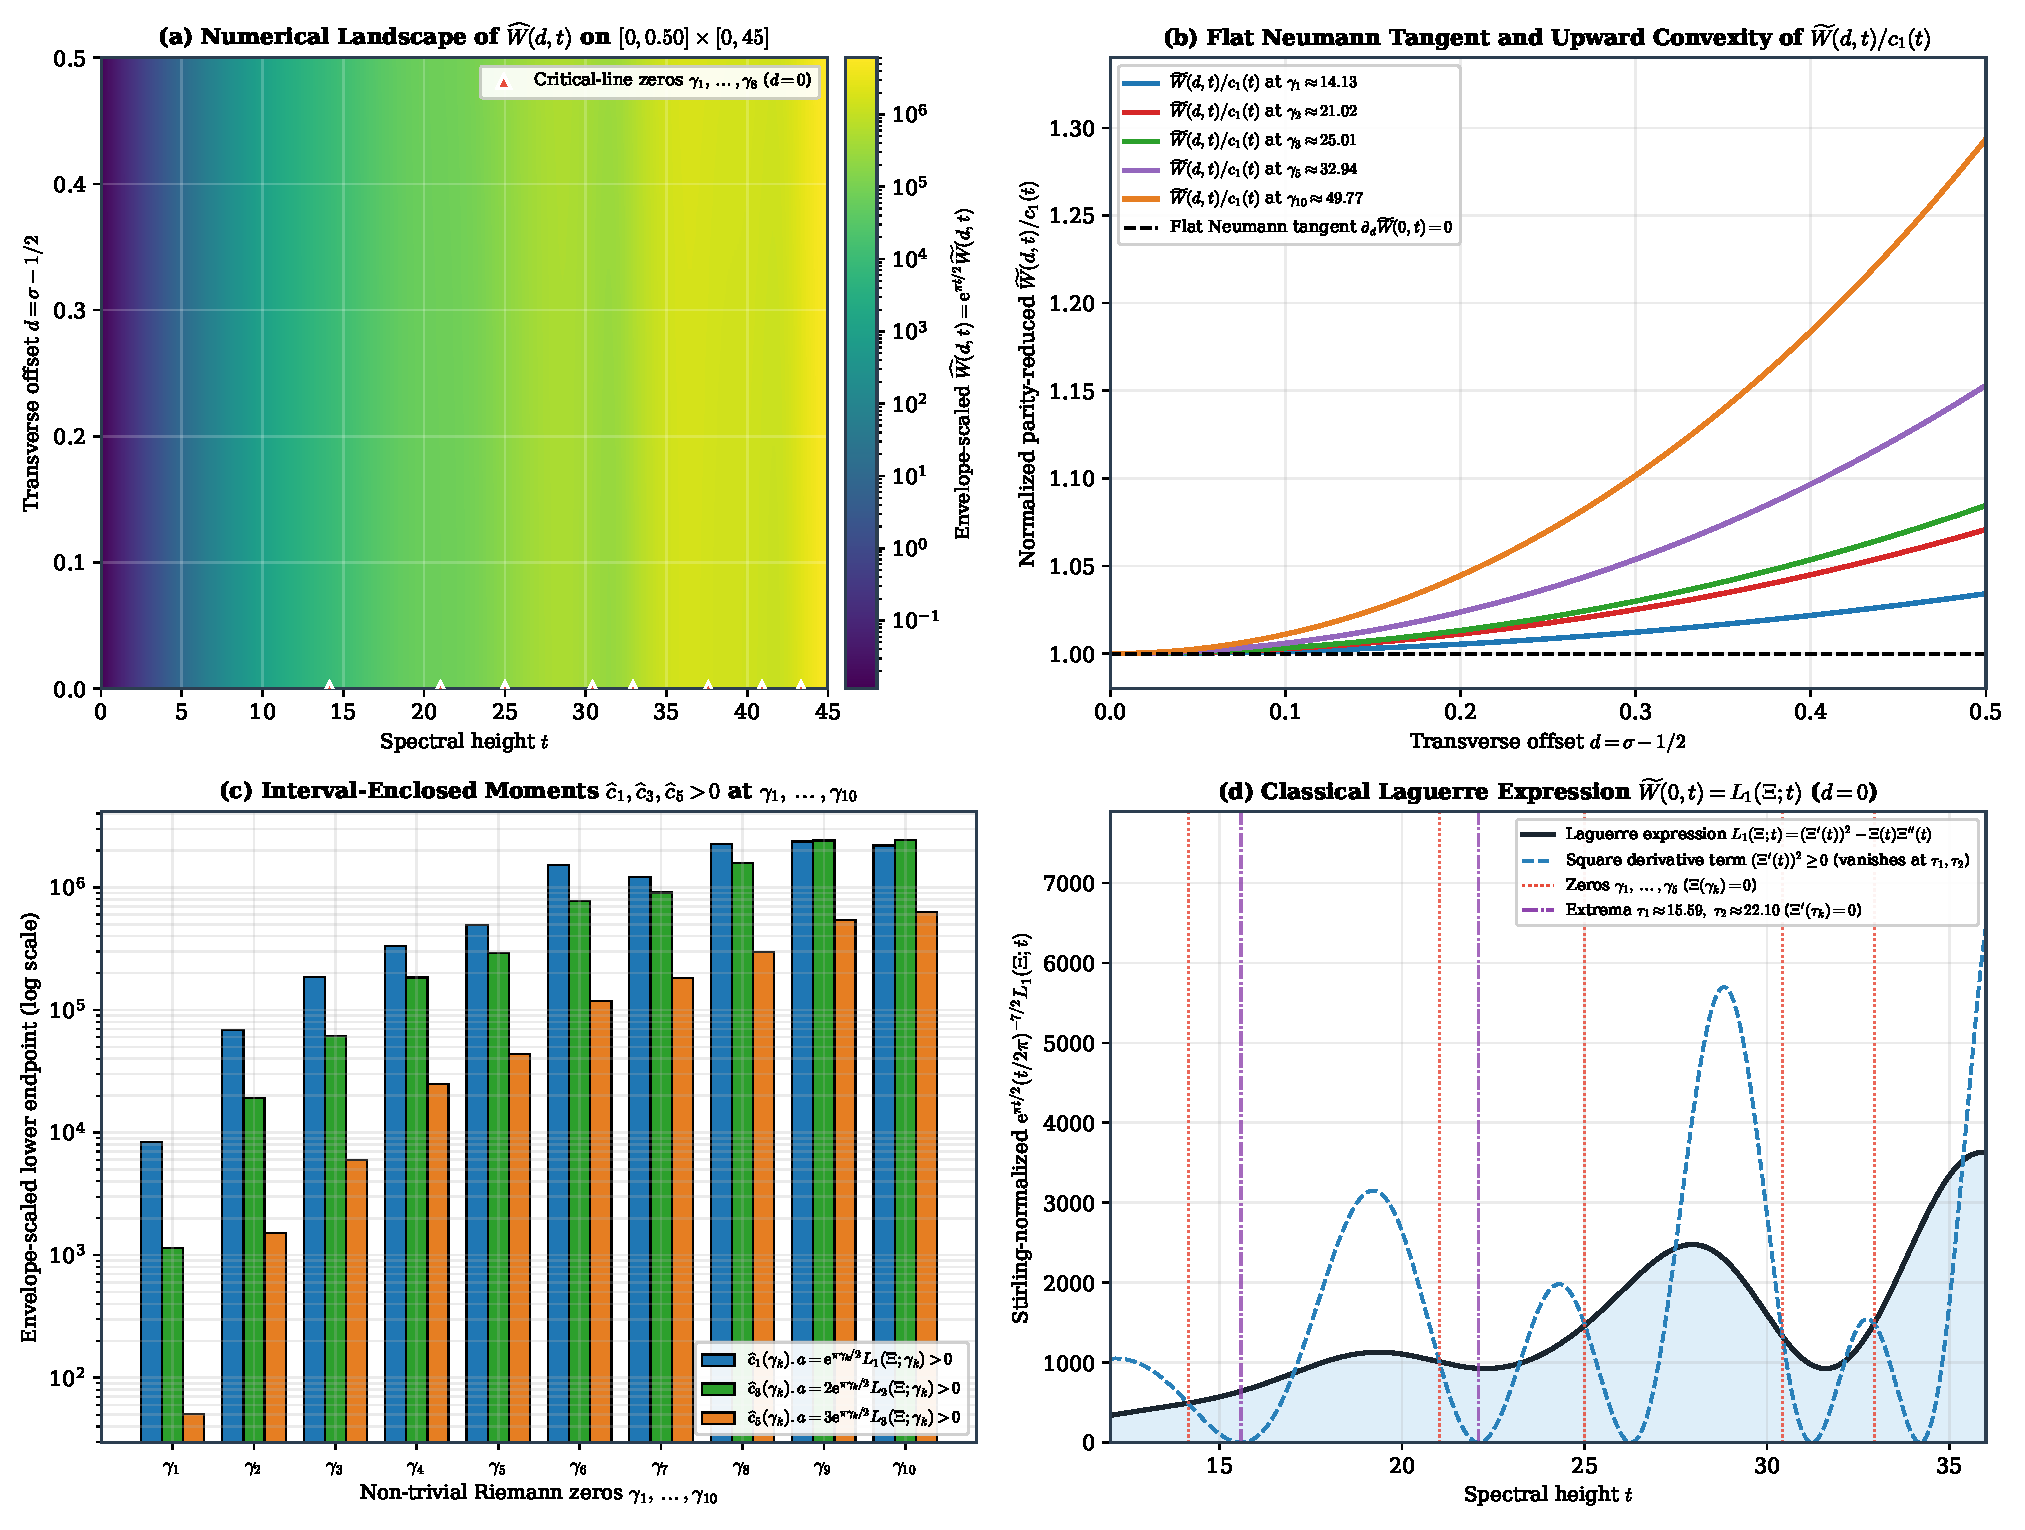
\includegraphics[width=0.94\textwidth]{figures/fig1_parity_reduced_wronskian_and_dipoles.pdf}
\caption{(a) Exploratory numerical landscape of $\What(d,t) = \ee^{\pi t/2}\Wtil(d,t)$ on $[0, 0.50] \times [0, 45]$ alongside critical-line zeros $\gamma_1, \dots, \gamma_8$. (b) Normalized profiles $\Wtil(d,t)/c_1(t)$ across $d \in [0, 0.50]$ showing the flat Neumann tangent $\partial_d\Wtil(0,t) = 0$. (c) Interval-enclosed moments $\widehat{c}_1(\boldsymbol{\gamma}_k).a, \widehat{c}_3(\boldsymbol{\gamma}_k).a, \widehat{c}_5(\boldsymbol{\gamma}_k).a > 0$ at $\gamma_1, \dots, \gamma_{10}$. (d) Classical Laguerre expression $\Wtil(0,t) = L_1(\Xi;t)$ versus $(\Xi'(t))^2$ on $t \in [12, 36]$, highlighting zeros $\gamma_k$ and true $\Xi'$-extrema $\tau_1 \approx 15.59$, $\tau_2 \approx 22.10$.}\label{fig:dipoles}
\end{figure}

\begin{figure}[htbp]
\centering
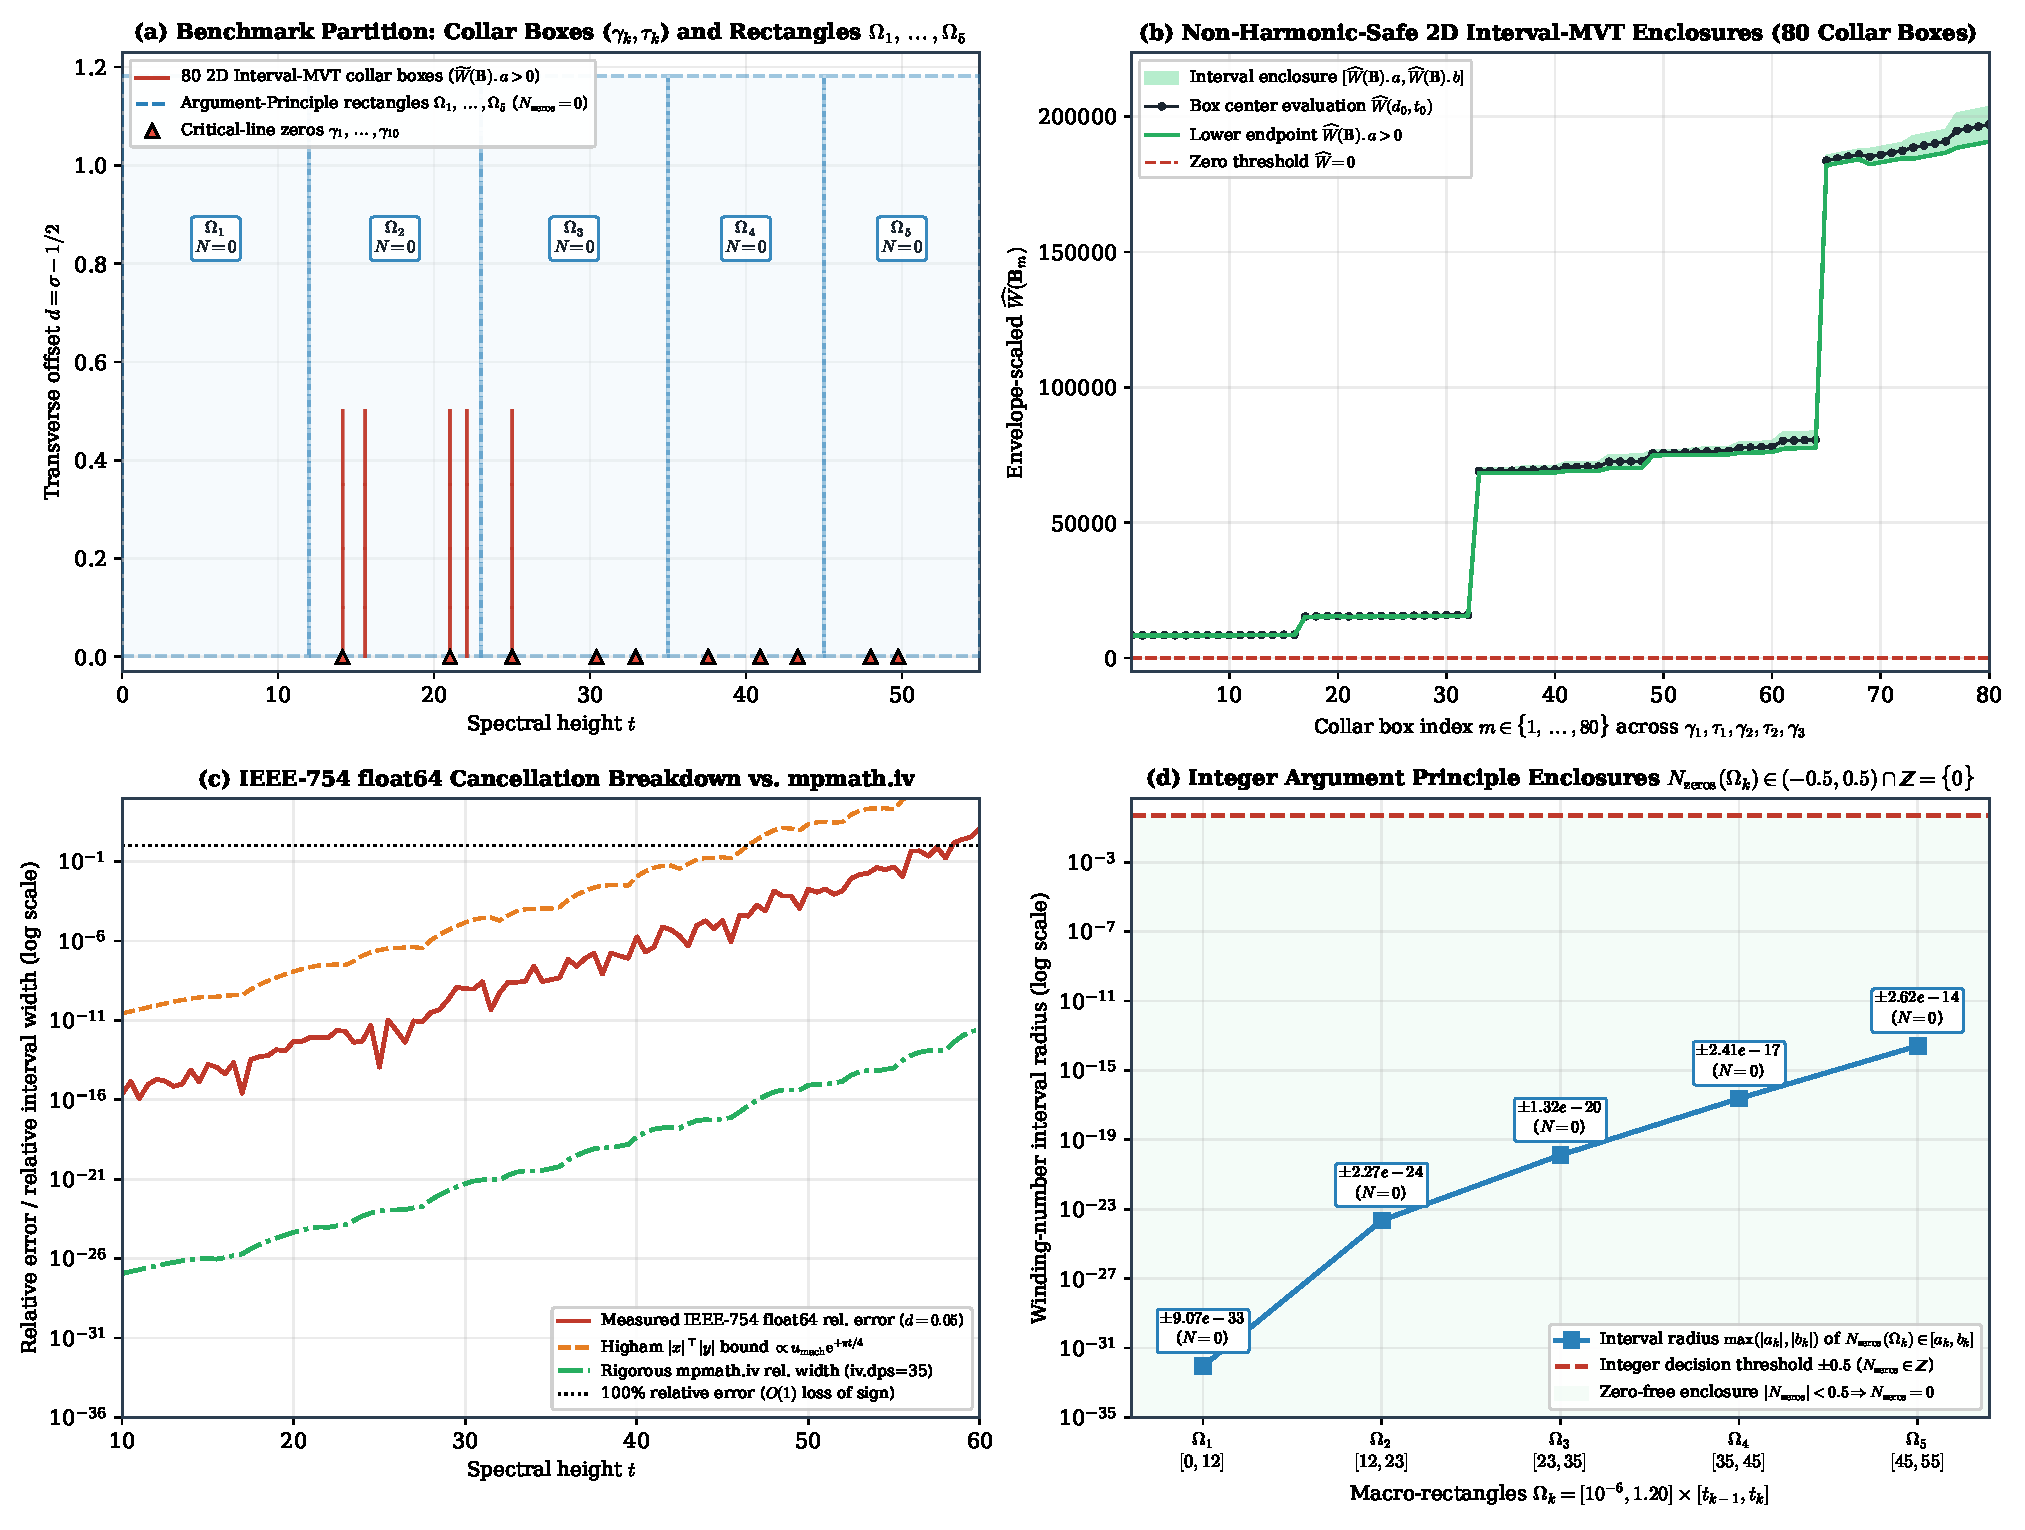
\includegraphics[width=0.94\textwidth]{figures/fig2_interval_mvt_and_argument_principle.pdf}
\caption{(a) Benchmark partition on $[0, 55]$: $80$ 2D Interval-MVT collar boxes $\mathbf{B}_m$ around $\gamma_k, \tau_k$ and five Cauchy rectangles $\Omega_1, \dots, \Omega_5$. (b) Non-harmonic-safe 2D Interval-MVT enclosures $[\What(\mathbf{B}_m).a, \What(\mathbf{B}_m).b]$ across Zones 1--5. (c) Exponential IEEE-754 \texttt{float64} relative error growth ($\propto u_{\mathrm{mach}}\ee^{+\pi t/4}$) versus Higham's $|x|^\top|y|$ bound and \texttt{mpmath.iv} (\texttt{iv.dps=35}) relative width across $t \in [10, 60]$. (d) Argument-principle winding radii $\max(|a_k|,|b_k|) \le 2.62 \times 10^{-14} < 0.5$ proving $N_{\mathrm{zeros}}(\Omega_k) = 0$.}\label{fig:interval_cert}
\end{figure}

\section{Scope, limitations, and explicit obstructions}\label{sec:scope}

We record the exact scope of the identities proved above and the structural obstructions separating finite-height interval benchmarks from asymptotic zero-free results:
\begin{enumerate}
\item \textbf{Davenport--Heilbronn and explicit off-critical zero counterexample ($L_1 < 0$):}
Proposition~\ref{prop:parity_wigner}, Theorem~\ref{thm:dipole_hierarchy}, and Proposition~\ref{prop:cr_gradients} use only Schwarz reflection $F(\bar{z}) = \overline{F(z)}$ and entireness (or Fourier decay), never the Euler product of $\zeta(s)$. Consequently, parity reduction $\Wtil_F(d,t) = W_F(d,t)/d$ and $c_{2m-1}(F;t) = m\,L_m(F;t)$ hold verbatim for the Davenport--Heilbronn function $\Xi_{\mathrm{DH}}(z)$ \cite{DavenportHeilbronn1936}, which satisfies the same $\Gamma$-functional equation as $\Xi$ yet has infinitely many zeros in $d > 0$, as well as for the explicit real-entire perturbation
\[
F_{\mathrm{off}}(z) := \Xi(z)\,\frac{(z^2 - z_*^2)(z^2 - \bar{z}_*^2)}{(z^2 - \gamma_1^2)(z^2 - \gamma_2^2)}, \qquad z_* = t_* - \ii d_*, \quad t_* = \tfrac{1}{2}(\gamma_1 + \gamma_2) \approx 17.5784, \quad d_* = 0.15.
\]
As verified to 50 decimal digits in the companion script (\nolinkurl{scripts/verify_paper2_parity_reduced_wronskian.py}), $\Wtil_{F_{\mathrm{off}}}(0, t_*) = L_1(F_{\mathrm{off}}; t_*) = -5.095559 \times 10^{-11} < 0$. By Csordas and Varga \cite{CsordasVarga1990}, proving $c_{2m-1}(t) = m\,L_m(\Xi;t) > 0$ globally for all $m \ge 1$ and $t \in \mathbb{R}$ is equivalent to RH, not an unconditional consequence of the $\sinch(2dy) \ge 1$ representation (since $I(y,t)$ oscillates in sign \cite{Missiaen2026Paper1}).
\item \textbf{Lehmer phenomenon and Skewes-scale Dirichlet phase alignment:}
At critical-line extrema $\Xi'(\tau_k) = 0$, $L_1(\Xi;\tau_k) = -\Xi(\tau_k)\Xi''(\tau_k)$ can become arbitrarily small whenever two zeros form a close Lehmer pair \cite{Lehmer1956}, requiring correspondingly finer interval boxes $\Delta t$ as logarithmic Dirichlet phases $\cos(t\log p)$ align coherently at large $t$.
\item \textbf{Voronin universality off the critical line:}
By Voronin's universality theorem \cite{Voronin1975}, on $\frac{1}{2} < \sigma < 1$ ($0 < d < \frac{1}{2}$) the shifts $\zeta(\sigma + \ii(t+\tau))$ approximate arbitrary non-vanishing holomorphic functions, ruling out any purely local Archimedean lower bound on $\Wtil(d,t)$ at large $t$ that ignores arithmetic cancellation.
\item \textbf{Exponential quadrature precision scaling ($\mathrm{dps}(T) \gtrsim \frac{\pi T}{4\ln 10}$):}
As quantified in Table~\ref{tab:float64_audit}, direct Fourier--Jacobi quadrature of \eqref{eq:Xi_integral} cancels $\approx \frac{\pi t}{4\ln 10} \approx 0.341\,t$ decimal digits, making large-height verification via raw $\Phi$-quadrature computationally prohibitive compared to FFT-accelerated Riemann--Siegel interval methods \cite{Platt2017,PlattTrudgian2021}.
\end{enumerate}

\appendix

\section{Explicit analytical error bounds for series, domain, and quadrature truncation}\label{app:bounds}

\begin{lemma}[Rigorous truncation bounds for interval evaluators]\label{lem:app_bounds}
Let $(d,t) \in [0, 1.20] \times [0, 55]$. Then:
\begin{enumerate}
\item[\textup{(a)}] \textbf{Power-series remainders near $w = 0$:} For $0 \le w \le 0.10$, truncating the Maclaurin series of $\cosh(w)$, $\sinch(w)$, and $\etah(w)$ after $w^{10}$ ($k = 5$) leaves non-negative remainders bounded by $1.01\frac{w^{12}}{12\fac}$, $1.01\frac{w^{12}}{13\fac}$, and $1.01\frac{14\,w^{12}}{15\fac}$, respectively.
\item[\textup{(b)}] \textbf{Euler--Maclaurin remainder \eqref{eq:em_rem_bound}:} For $\sigma = \frac{1}{2}+d > 0$ and integers $N, M \ge 1$, $|R_{M,N}(s)| \le \varepsilon_{\mathrm{EM}}(s)$.
\item[\textup{(c)}] \textbf{Jacobi series, domain tail, and strip trapezoidal bounds \eqref{eq:trunc_summary}:} For $M_{\mathrm{ser}} = 12$, $U_{\max} = 1.55$, and $h = 1.55/140$, the truncation errors across all auxiliary integrals in \eqref{eq:Xi_integral} and \eqref{eq:aux_integrals} satisfy $\varepsilon_{\mathrm{ser}} \le 10^{-220}$, $\varepsilon_{\mathrm{tail}} \le 10^{-550}$, and $\varepsilon_{\mathrm{quad}} \le 10^{-55}$.
\end{enumerate}
\end{lemma}

\begin{proof}
Parts~(a) and (b) follow respectively from geometric majorization with term ratio $\frac{w^2}{13 \cdot 14} < 10^{-4}$ and the standard Euler--Maclaurin remainder theorem \cite[Section~6.4]{Titchmarsh1986}. For part~(c), for $u \ge 0$ and $n \ge 13$, $\pi n^2 \ee^{4u} \ge 169\pi > 530.9$, giving $\varepsilon_{\mathrm{ser}} \le 16\pi^2(13^4)\ee^{-169\pi} < 10^{-220}$; for $u \ge 1.55$ and $d \le 1.20$, $\pi\ee^{4u} > 1548.8$ while $(2u)^8\cosh(2du)\ee^{9u} < 4.2 \times 10^{11}$, giving $\varepsilon_{\mathrm{tail}} < 10^{-550}$. Finally, $\Phi(u)$ is even and holomorphic throughout the open strip $|\Ima(u)| < \frac{\pi}{8} \approx 0.3927$ (note that the strip zeros of $\Phi$ at $\pm\ii\tau_0 \approx \pm 0.3194\ii$ and $\pm 0.1278 \pm 0.3478\ii$ analyzed in \cite{Missiaen2026Paper1} create logarithmic singularities for $\log\Phi$ in saddle-point asymptotics, not poles of the holomorphic integrand $\Phi(u)(2u)^m\cosh(2du)\cos(2tu)$). On $|\Ima(u)| \le \eta = 0.35 < \frac{\pi}{8}$, $\cos(4\eta) \approx 0.16997 > 0$ gives double-exponential decay as $\Rea(u) \to \pm\infty$. By \cite[Theorem~5.1]{TrefethenWeideman2014}, $\varepsilon_{\mathrm{quad}}(h) \le 2 M(\eta)\ee^{2(|t|+|d|)\eta}/(\ee^{2\pi\eta/h} - 1)$ with $2\pi\eta/h = 2\pi(0.35)(140)/1.55 \approx 198.63$, $\ee^{-2\pi\eta/h} \approx 5.45 \times 10^{-87}$, $\ee^{2(55+1.20)(0.35)} \approx 1.22 \times 10^{17}$, and $M(0.35) \le 10^{12}$, yielding $\varepsilon_{\mathrm{quad}}(h) < 10^{-55}$.
\end{proof}

\section*{Use of AI and Computational Tools}

\textbf{Gemini} (Google DeepMind) was used interactively to assist with symbolic verification of the positive-weight integral majorants, algebraic cross-checking against the classical Jensen--Csordas--Varga identities, and implementation of the Python \texttt{mpmath.iv} interval benchmark and IEEE-754 cancellation audit (\nolinkurl{scripts/verify_paper2_parity_reduced_wronskian.py}). All analytical proofs, error bounds, citations, and numerical outputs were independently checked and verified.

\begin{thebibliography}{99}

\bibitem{Csordas1986}
G.~Csordas, T.~S.~Norfolk, and R.~S.~Varga, \emph{The Riemann hypothesis and the Tur\'an inequalities}, Trans. Amer. Math. Soc. \textbf{296} (1986), no.~2, 521--541.

\bibitem{CsordasVarga1990}
G.~Csordas and R.~S.~Varga, \emph{Necessary and sufficient conditions and the Riemann hypothesis}, Adv. Appl. Math. \textbf{11} (1990), no.~3, 328--357.

\bibitem{DavenportHeilbronn1936}
H.~Davenport and H.~Heilbronn, \emph{On the zeros of certain Dirichlet series. I, II}, J. London Math. Soc. \textbf{11} (1936), 181--185, 307--312.

\bibitem{Gram1903}
J.-P.~Gram, \emph{Note sur les z\'eros de la fonction $\zeta(s)$ de Riemann}, Acta Math. \textbf{27} (1903), 289--304.

\bibitem{Griffin2019}
M.~Griffin, K.~Ono, L.~Rolen, and D.~Zagier, \emph{Jensen polynomials for the Riemann zeta function and other sequences}, Proc. Natl. Acad. Sci. USA \textbf{116} (2019), no.~23, 11103--11110.

\bibitem{Higham2002}
N.~J.~Higham, \emph{Accuracy and Stability of Numerical Algorithms}, 2nd ed., Society for Industrial and Applied Mathematics (SIAM), Philadelphia, PA, 2002.

\bibitem{Hinkkanen1997}
A.~Hinkkanen, \emph{On functions of bounded type}, Complex Variables Theory Appl. \textbf{34} (1997), no.~1--2, 119--139.

\bibitem{Jensen1913}
J.~L.~W.~V.~Jensen, \emph{Recherches sur la th\'eorie des \'equations}, Acta Math. \textbf{36} (1913), 181--195.

\bibitem{Lagarias1999}
J.~C.~Lagarias, \emph{On a positivity property of the Riemann $\xi$-function}, Acta Arith. \textbf{89} (1999), no.~3, 217--234.

\bibitem{Lehmer1956}
D.~H.~Lehmer, \emph{Extended computation of the Riemann zeta-function}, Mathematika \textbf{3} (1956), 102--108.

\bibitem{Missiaen2026Paper1}
T.~Missiaen, \emph{Wigner Phase-Space Representation, Shifted Cauchy Contours, and Local Saddle-Point Coalescence in the Transverse Wronskian of Riemann's $\Xi$-Function}, Preprint, Zenodo (2026), DOI: \href{https://doi.org/10.5281/zenodo.23637324}{10.5281/zenodo.23637324}.

\bibitem{Platt2017}
D.~J.~Platt, \emph{Isolating some non-trivial zeros of zeta}, Math. Comp. \textbf{86} (2017), no.~307, 2449--2467.

\bibitem{PlattTrudgian2021}
D.~J.~Platt and T.~S.~Trudgian, \emph{The Riemann hypothesis is true up to $3\cdot 10^{12}$}, Bull. Lond. Math. Soc. \textbf{53} (2021), no.~3, 792--797.

\bibitem{Polya1926}
G.~P\'olya, \emph{Bemerkung \"uber die Integraldarstellung der Riemannschen $\xi$-Funktion}, Acta Math. \textbf{48} (1926), 305--317.

\bibitem{Polya1927}
G.~P\'olya, \emph{\"Uber die algebraisch-funktionentheoretischen Untersuchungen von J.~L.~W.~V.~Jensen}, Kgl. Danske Vid. Sel. Math.-Fys. Medd. \textbf{7} (1927), no.~17, 3--33.

\bibitem{Riemann1859}
B.~Riemann, \emph{Ueber die Anzahl der Primzahlen unter einer gegebenen Gr\"osse}, Monatsberichte der Berliner Akademie (1859), 671--680.

\bibitem{Speiser1934}
A.~Speiser, \emph{Geometrisches zur Riemannschen Zetafunktion}, Math. Ann. \textbf{110} (1934), no.~1, 514--521.

\bibitem{Spira1968}
R.~Spira, \emph{Zeros of $\zeta'(s)$ in the critical strip}, Math. Comp. \textbf{22} (1968), 163--173.

\bibitem{Spira1973}
R.~Spira, \emph{Zeros of $\zeta'(s)$ and the Riemann hypothesis}, Illinois J. Math. \textbf{17} (1973), 147--152.

\bibitem{TitchmarshComrie1936}
E.~C.~Titchmarsh, \emph{The zeros of the Riemann zeta-function}, Proc. Roy. Soc. London Ser. A \textbf{151} (1935), 234--255; \textbf{157} (1936), 261--263.

\bibitem{Titchmarsh1986}
E.~C.~Titchmarsh, \emph{The Theory of the Riemann Zeta-Function}, 2nd ed., edited and with a preface by D.~R.~Heath-Brown, Oxford University Press, Oxford, 1986.

\bibitem{TrefethenWeideman2014}
L.~N.~Trefethen and J.~A.~C.~Weideman, \emph{The exponentially convergent trapezoidal rule}, SIAM Rev. \textbf{56} (2014), no.~3, 385--458.

\bibitem{Turing1953}
A.~M.~Turing, \emph{Some calculations of the Riemann zeta-function}, Proc. London Math. Soc. (3) \textbf{3} (1953), 99--117.

\bibitem{Voronin1975}
S.~M.~Voronin, \emph{Theorem on the ``universality'' of the Riemann zeta-function}, Math. USSR-Izv. \textbf{9} (1975), no.~3, 443--453.

\end{thebibliography}

\end{document}
